%----------
%   IMPORTANTE
%----------

% Si nunca has utilizado LaTeX es conveniente que aprendas una serie de conceptos básicos antes de utilizar esta plantilla. Te aconsejamos que leas previamente algún tutorial (puedes encontar muchos en Internet).

% Esta plantilla está basada en las recomendaciones de la guía "Trabajo fin de Grado: Escribir el TFG", que encontrarás en http://uc3m.libguides.com/TFG/escribir
% contiene recomendaciones de la Biblioteca basadas principalmente en estilos APA e IEEE, pero debes seguir siempre las orientaciones de tu Tutor de TFG y la normativa de TFG para tu titulación.

% Encontrarás un ejemplo de TFG realizado con esta misma plantilla en la carpeta "_ejemplo_TFG_2019". Consúltalo porque contiene ejemplos útiles para incorporar tablas, figuras, listados de código, bibliografía, etc.


%----------
%	CONFIGURACIÓN DEL DOCUMENTO
%----------

% Definimos las características del documento y añadimos una serie de paquetes (\usepackage{package}) que agregan funcionalidades a LaTeX.

\documentclass[12pt]{report} %fuente a 12pt

% MÁRGENES: 2,5 cm sup. e inf.; 3 cm izdo. y dcho.
\usepackage[
a4paper,
vmargin=2.5cm,
hmargin=3cm
]{geometry}

% INTERLINEADO: Estrecho (6 ptos./interlineado 1,15) o Moderado (6 ptos./interlineado 1,5)
\renewcommand{\baselinestretch}{1.15}
\parskip=6pt

% DEFINICIÓN DE COLORES para portada y listados de código
\usepackage[table]{xcolor}
\definecolor{azulUC3M}{RGB}{0,0,102}
\definecolor{gray97}{gray}{.97}
\definecolor{gray75}{gray}{.75}
\definecolor{gray45}{gray}{.45}

% Soporte para GENERAR PDF/A --es importante de cara a su inclusión en e-Archivo porque es el formato óptimo de preservación y a la generación de metadatos, tal y como se describe en http://uc3m.libguides.com/ld.php?content_id=31389625. En la carpeta incluímos el archivo plantilla_tfg_2017.xmpdata en el que puedes incluir los metadatos que se incorporarán al archivo PDF cuando lo compiles. Ese archivo debe llamarse igual que tu archivo .tex. Puedes ver un ejemplo en esta misma carpeta.
\usepackage[a-1b]{pdfx}

% ENLACES
\usepackage{hyperref}
\hypersetup{colorlinks=true,
	linkcolor=black, % enlaces a partes del documento (p.e. índice) en color negro
	urlcolor=blue} % enlaces a recursos fuera del documento en azul

\usepackage{booktabs}


% EXPRESIONES MATEMATICAS
\usepackage{amsmath,amssymb,amsfonts,amsthm}
\usepackage{txfonts} 
\usepackage[T1]{fontenc}
\usepackage[utf8]{inputenc}

\usepackage[spanish, es-tabla]{babel} 
\usepackage[babel, spanish=spanish]{csquotes}
\AtBeginEnvironment{quote}{\small}

% diseño de PIE DE PÁGINA
\usepackage{fancyhdr}
\pagestyle{fancy}
\fancyhf{}
\renewcommand{\headrulewidth}{0pt}
\rfoot{\thepage}
\fancypagestyle{plain}{\pagestyle{fancy}}


% DISEÑO DE LOS TÍTULOS de las partes del trabajo (capítulos y epígrafes o subcapítulos)
\usepackage{titlesec}
\usepackage{titletoc}
\titleformat{\chapter}[block]
{\large\bfseries\filcenter}
{\thechapter.}
{5pt}
{\MakeUppercase}
{}
\titlespacing{\chapter}{0pt}{0pt}{*3}
\titlecontents{chapter}
[0pt]                                               
{}
{\contentsmargin{0pt}\thecontentslabel.\enspace\uppercase}
{\contentsmargin{0pt}\uppercase}                        
{\titlerule*[.7pc]{.}\contentspage}

\titleformat{\section}
{\bfseries}
{\thesection.}
{5pt}
{}
\titlecontents{section}
[5pt]                                               
{}
{\contentsmargin{0pt}\thecontentslabel.\enspace}
{\contentsmargin{0pt}}
{\titlerule*[.7pc]{.}\contentspage}

\titleformat{\subsection}
{\normalsize\bfseries}
{\thesubsection.}
{5pt}
{}
\titlecontents{subsection}
[10pt]                                               
{}
{\contentsmargin{0pt}                          
	\thecontentslabel.\enspace}
{\contentsmargin{0pt}}                        
{\titlerule*[.7pc]{.}\contentspage}  


% DISEÑO DE TABLAS. Puedes elegir entre el estilo para ingeniería o para ciencias sociales y humanidades. Por defecto, está activado el estilo de ingeniería. Si deseas utilizar el otro, comenta las líneas del diseño de ingeniería y descomenta las del diseño de ciencias sociales y humanidades
\usepackage{multirow} % permite combinar celdas 
\usepackage{caption} % para personalizar el título de tablas y figuras
\usepackage{floatrow} % utilizamos este paquete y sus macros \ttabbox y \ffigbox para alinear los nombres de tablas y figuras de acuerdo con el estilo definido. Para su uso ver archivo de ejemplo 
\usepackage{array} % con este paquete podemos definir en la siguiente línea un nuevo tipo de columna para tablas: ancho personalizado y contenido centrado
\newcolumntype{P}[1]{>{\centering\arraybackslash}p{#1}}
\DeclareCaptionFormat{upper}{#1#2\uppercase{#3}\par}

% Diseño de tabla para ingeniería
\captionsetup[table]{
	format=upper,
	name=TABLA,
	justification=centering,
	labelsep=period,
	width=.75\linewidth,
	labelfont=small,
	font=small,
}

%Diseño de tabla para ciencias sociales y humanidades
%\captionsetup[table]{
%	justification=raggedright,
%	labelsep=period,
%	labelfont=small,
%	singlelinecheck=false,
%	font={small,bf}
%}


% DISEÑO DE FIGURAS. Puedes elegir entre el estilo para ingeniería o para ciencias sociales y humanidades. Por defecto, está activado el estilo de ingeniería. Si deseas utilizar el otro, comenta las líneas del diseño de ingeniería y descomenta las del diseño de ciencias sociales y humanidades
\usepackage{graphicx}
\usepackage{subcaption}
\graphicspath{{imagenes/}} %ruta a la carpeta de imágenes

% Diseño de figuras para ingeniería
\captionsetup[figure]{
	format=hang,
	name=Fig.,
	singlelinecheck=off,
	labelsep=period,
	labelfont=small,
	font=small		
}

% Diseño de figuras para ciencias sociales y humanidades
%\captionsetup[figure]{
%	format=hang,
%	name=Figura,
%	singlelinecheck=off,
%	labelsep=period,
%	labelfont=small,
%	font=small		
%}


% NOTAS A PIE DE PÁGINA
\usepackage{chngcntr} %para numeración contínua de las notas al pie
\counterwithout{footnote}{chapter}

% LISTADOS DE CÓDIGO
% soporte y estilo para listados de código. Más información en https://es.wikibooks.org/wiki/Manual_de_LaTeX/Listados_de_código/Listados_con_listings
\usepackage{listings}

% definimos un estilo de listings
\lstdefinestyle{estilo}{ frame=Ltb,
	framerule=0pt,
	aboveskip=0.5cm,
	framextopmargin=3pt,
	framexbottommargin=3pt,
	framexleftmargin=0.4cm,
	framesep=0pt,
	rulesep=.4pt,
	backgroundcolor=\color{gray97},
	rulesepcolor=\color{black},
	%
	basicstyle=\ttfamily\footnotesize,
	keywordstyle=\bfseries,
	stringstyle=\ttfamily,
	showstringspaces = false,
	commentstyle=\color{gray45},     
	%
	numbers=left,
	numbersep=15pt,
	numberstyle=\tiny,
	numberfirstline = false,
	breaklines=true,
	xleftmargin=\parindent
}

\captionsetup[lstlisting]{font=small, labelsep=period}
% fijamos el estilo a utilizar 
\lstset{style=estilo}
\renewcommand{\lstlistingname}{\uppercase{Código}}


%BIBLIOGRAFÍA - PUEDES ELEGIR ENTRE ESTILO IEEE O APA. POR DEFECTO ESTÁ CONFIGURADO IEEE. SI DESEAS USAR APA, COMENTA LAS LÍNEA DE IEEE Y DESCOMENTA LAS DE APA. Si haces cambios en la configuración de la bibliografía y no obtienes los resultados esperados, es recomendable limpiar los archivos auxiliares y volver a compilar en este orden: COMPILAR-BIBLIOGRAFIA-COMPILAR

% Tienes más información sobre cómo generar bibliografía y CONFIGURAR TU EDITOR DE TEXTO para compilar con biber en http://tex.stackexchange.com/questions/154751/biblatex-with-biber-configuring-my-editor-to-avoid-undefined-citations , https://www.overleaf.com/learn/latex/Bibliography_management_in_LaTeX y en http://www.ctan.org/tex-archive/macros/latex/exptl/biblatex-contrib
% También te recomendamos consultar la guía temática de la Biblioteca sobre citas bibliográficas: http://uc3m.libguides.com/guias_tematicas/citas_bibliograficas/inicio

% CONFIGURACIÓN PARA LA BIBLIOGRAFÍA IEEE
\usepackage[backend=biber, style=ieee, isbn=false,sortcites, maxbibnames=5, minbibnames=1]{biblatex} % Configuración para el estilo de citas de IEEE, recomendado para el área de ingeniería. "maxbibnames" indica que a partir de 5 autores trunque la lista en el primero (minbibnames) y añada "et al." tal y como se utiliza en el estilo IEEE.

%CONFIGURACIÓN PARA LA BIBLIOGRAFÍA APA
%\usepackage[style=apa, backend=biber, natbib=true, hyperref=true, uniquelist=false, sortcites]{biblatex}
%\DeclareLanguageMapping{spanish}{spanish-apa}

% Añadimos las siguientes indicaciones para mejorar la adaptación de los estilos en español
\DefineBibliographyStrings{spanish}{%
	andothers = {et\addabbrvspace al\adddot}
}
\DefineBibliographyStrings{spanish}{
	url = {\adddot\space[En línea]\adddot\space Disponible en:}
}
\DefineBibliographyStrings{spanish}{
	urlseen = {Acceso:}
}
\DefineBibliographyStrings{spanish}{
	pages = {pp\adddot},
	page = {p.\adddot}
}

\addbibresource{bibliografia/bibliografia.bib} % llama al archivo bibliografia.bib en el que debería estar la bibliografía utilizada


%-------------
%	DOCUMENTO
%-------------

\begin{document}
\pagenumbering{roman} % Se utilizan cifras romanas en la numeración de las páginas previas al cuerpo del trabajo
	
%----------
%	PORTADA
%----------	
\begin{titlepage}
	\begin{sffamily}
	\color{azulUC3M}
	\begin{center}
		\begin{figure}[H] %incluimos el logotipo de la Universidad
			\makebox[\textwidth][c]{
\includegraphics[width=16cm]{Portada_Logo.png}}
		\end{figure}
		\vspace{2.5cm}
		\begin{Large}
			Grado en Ingeniería Informática\\			
			2022-2023\\
			\vspace{2cm}		
			\textsl{Trabajo Fin de Grado}
			\bigskip
			
		\end{Large}
		 	{\Huge ``Sistema de Recomendación de Moda basado en Atributos Multimodales''}\\
		 	\vspace*{0.5cm}
	 		\rule{10.5cm}{0.1mm}\\
			\vspace*{0.9cm}
			{\LARGE Gonzalo Llosá Cea}\\ 
			\vspace*{1cm}
		\begin{Large}
			Tutores\\
			Miguel Ángel Patricio Guisado\\
			Carlos Rodríguez - Pardo\\
			Madrid, septiembre\\
		\end{Large}
	\end{center}
	\vfill
	\color{black}
	% si nuestro trabajo se va a publicar con una licencia Creative Commons, incluir estas líneas. Es la opción recomendada.
	
\includegraphics[width=4.2cm]{imagenes/creativecommons.png}\\ %incluimos el logotipo de creativecommons
	Esta obra se encuentra sujeta a la licencia Creative Commons \textbf{Reconocimiento - No Comercial - Sin Obra Derivada}
	\end{sffamily}
\end{titlepage}

\newpage %página en blanco o de cortesía
\thispagestyle{empty}
\mbox{}

%----------
%	RESUMEN Y PALABRAS CLAVE
%----------	
\renewcommand\abstractname{\large\bfseries\filcenter\uppercase{Resumen}}
\begin{abstract}
\thispagestyle{plain}
\setcounter{page}{3}
	
	% ESCRIBIR EL RESUMEN AQUÍ
	La industria de la moda es una de las más potentes en nuestro país y esta se ha ido adaptando al auge tecnológico
	que hemos vivido en las últimas décadas. Un gran porcentaje de las ventas de este sector se realizan de manera
	online y es por ello la importancia de un sistema de recomendación.
	
	Un sistema de recomendación de moda para las tiendas online resulta muy beneficioso, tanto para propietarios como
	para clientes. Los primeros aumentan sus ventas mientras que los segundos encuentran más fácil y rápido productos
	que, en muchas ocasiones, ni siquiera hubieran podido encontrar.

	Para solucionar este problema se hace uso de una amplia base de datos en donde las prendas vienen etiquetadas por sus
	diferentes atributos. Después de realizar un estudio sobre las tecnologías que pueden resolver este problema, se eligen
	diferentes arquitecturas para resolver las diferentes partes que componen el objetivo principal. Para la segmentación de
	imágenes, con el fin de conseguir sus máscaras, se hace uso de la arquitectura U2-Net. Para el algoritmo de recomendación,
	se extraen los vectores de características de las imágenes haciendo uso de la arquitectura VGG16, para posteriormente 
	calcular la similitud coseno entre estos vectores. Además se añade la posibilidad de elegir los atributos que se quieren
	presentes en la recomendación de la prenda.  

	Una vez se realiza este modelo se desarrolla una aplicación web que es capaz de servirlo para que los usuarios puedan utilizarlo
	de una manera fácil e intuitiva. El modelo se sirve a través de una API, haciendo uso de \textit{Flask}, a la aplicación web 
	hecha con \textit{React}.

	También se lleva a cabo un estudio de la efectividad del sistema, analizando los porcentajes de similitud entre recomendaciones
	y la calidad de estas.

	Este proyecto tiene gran relevancia en el mundo real. Puede llegar a causar un gran impacto tanto en clientes de negocios
	de venta online de ropa como en los propios clientes.

	\textbf{Palabras clave:}
	% Escribir las palabras clave aquí
	Red convolucional, visión por computadora, segmentación de imágenes, interfaz gráfica.
	\vfill

\end{abstract}
	\newpage % página en blanco o de cortesía
	\thispagestyle{empty}
	\mbox{}


	\renewcommand\abstractname{\large\bfseries\filcenter\uppercase{abstract}}
	\begin{abstract}
	\thispagestyle{plain}
	\setcounter{page}{3}
		
		% ESCRIBIR EL RESUMEN AQUÍ
		The fashion industry is one of the most powerful sectors in our country, and it has been adapting to the technological boom that we have experienced in recent decades. A significant percentage of sales in this sector occur online, underscoring the importance of a recommendation system.

		A fashion recommendation system for online stores proves highly advantageous, benefiting both proprietors and customers. The former witness an increase in sales, while the latter find it easier and quicker to discover products that, in many instances, they might not have come across otherwise.
		
		To address this issue, an extensive database is employed, wherein garments are labeled with their distinct attributes. After conducting a study on technologies capable of resolving this problem, diverse architectures are selected to tackle the various components constituting the primary objective. For image segmentation, aimed at obtaining their masks, the U2-Net architecture is utilized. Concerning the recommendation algorithm, feature vectors are extracted from the images using the VGG16 architecture, subsequently computing the cosine similarity between these vectors. Furthermore, the option to select the attributes to be present in the garment recommendation is incorporated.
		
		Once this model is developed, a web application is created to facilitate user-friendly and intuitive utilization. The model is served through an API, utilizing \textit{Flask}, for the web application built with \textit{React}.
		
		An assessment of the system's effectiveness is also conducted, analyzing similarity percentages between recommendations and their quality.
		
		This project holds significant relevance in the real world, potentially yielding a substantial impact on both the clientele of online clothing businesses and the customers themselves.
	
		\textbf{Keywords:}
		% Escribir las palabras clave aquí
		Convolutional network, computer vision, images segmentation, graphic interface.
		Red convolucional, visión por computadora, segmentación de imágenes, interfaz gráfica.
		\vfill

	\end{abstract}

\newpage % página en blanco o de cortesía
\thispagestyle{empty}
\mbox{}

%----------
%	DEDICATORIA
%----------	
% \chapter*{Dedicatoria}

% \setcounter{page}{5}
	
% 	% ESCRIBIR LA DEDICATORIA AQUÍ	
		
% 	\vfill
	
% 	\newpage % página en blanco o de cortesía
% 	\thispagestyle{empty}
% 	\mbox{}
	

%----------
%	ÍNDICES
%----------	

%--
% Índice general
%-
\tableofcontents
\thispagestyle{fancy}

\newpage % página en blanco o de cortesía
\thispagestyle{empty}
\mbox{}

%--
% Índice de figuras. Si no se incluyen, comenta las líneas siguientes
%-
\listoffigures
\thispagestyle{fancy}

\newpage % página en blanco o de cortesía
\thispagestyle{empty}
\mbox{}

%--
% Índice de tablas. Si no se incluyen, comenta las líneas siguientes
%-
\listoftables
\thispagestyle{fancy}

\newpage % página en blanco o de cortesía
\thispagestyle{empty}
\mbox{}

\chapter*{Lista de Acrónimos}
\begin{center}
	\begin{tabular}{c p{8cm}} % Ajusta el ancho de la columna de los acrónimos según tus necesidades
			API & Application Programming Interface \\
			PIB & Producto Interior Bruto \\
			HTML & HyperText Markup Language \\
			CSS & Cascading Style Sheets \\
			CPU & Central Processing Unit \\
			GPU & Graphics Processing Unit \\
			IDE & Integrated development environment \\
			UI & User Interface
	\end{tabular}
\end{center}

\newpage % página en blanco o de cortesía
\thispagestyle{empty}
\mbox{}


%----------
%	TRABAJO
%----------	
\clearpage
\pagenumbering{arabic} % numeración con múmeros arábigos para el resto de la publicación	

\chapter{Introducción}

	% COMENZAR A ESCRIBIR EL TRABAJO
	\section{Motivación}
	La industria de la moda siempre ha sido una de las más potentes en nuestra sociedad.
	Esta industria se ha ido adaptando al auge que han tenido las tecnologías informáticas
	y es que, en el año 2022, las ventas de ropa online supusieron el 21,1\% de las ventas
	totales en nuestro país. 
	\begin{figure}[H]
		\ffigbox[\FBwidth]
		{\caption[Peso de las ventas moda online sobre el total de los ingresos generados por las ventas de ropa en España de 2012 a 2022]{Peso de las ventas moda online sobre el total de los ingresos generados por las ventas de ropa en España de 2012 a 2022 \cite{statista}}}
		{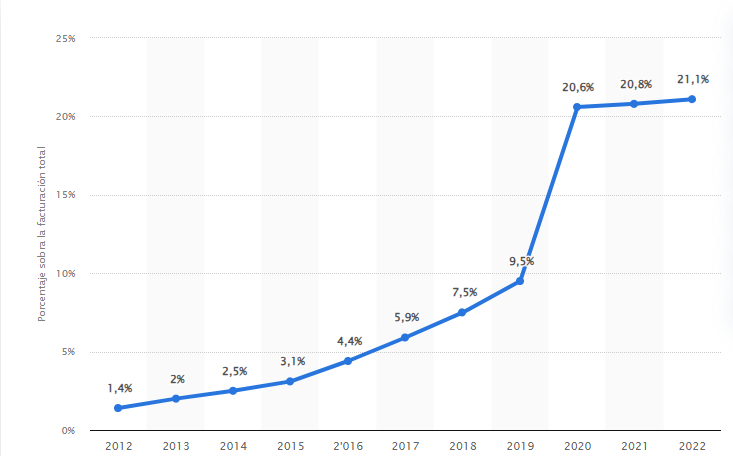
\includegraphics[scale=0.6]{venta-online-moda.png}}
	\end{figure}
	Es aquí donde entran en juego los sistemas de recomendación.
	Un sistema de recomendación de moda permite ayudar a las personas a encontrar prendas
	que se ajusten a sus gustos. 
	Los clientes pueden mejorar su experiencia de compra y estar satisfechos con sus elecciones 
	al recibir recomendaciones personalizadas y precisas. Esto resulta en un aumento
	de las ventas de los sitios web que se dedican a la moda.
	Un sistema de recomendación que esté basado únicamente en imágenes es útil, pero el hecho de
	introducir la posibilidad de especificar los atributos que deben estar en las prendas lo mejora
	aún más. Permitir a los usuarios obtener recomendaciones les ahorra mucho tiempo en búsquedas
	que, en muchas ocasiones, pueden resultar tediosas.

	En conclusión, el hecho de crear un sistema de recomendación de moda basado en atributos multimodales
	resulta muy interesante tanto para propietarios de tiendas online, ya que mejoran sus ventas, como para
	usuarios, que tienen más facilidad a la hora de encontrar las prendas que buscan, ahorrando así una
	gran cantidad de tiempo.

	\section{Objetivos}
	El objetivo de este trabajo es el de crear una interfaz web que sea capaz de recomendar imágenes de
	ropa, con una cierta similitud, a partir de otra previamente dada por el usuario. Además se podrán 
	especificar los atributos que se deseen en las imágenes de salida (por ejemplo: manga larga, ajuste suelto, etc.).
	\\
	Siendo este el principal objetivo podemos diferenciar los siguientes sub-objetivos:
	\begin{itemize}
		\item Desarrollar un modelo de inteligencia artificial que sea capaz de recomendar imágenes en base a atributos multimodales y otra imagen.
		\item Crear una API que permita la comunicación entre el modelo previamente mencionado y una interfaz.
		\item Diseñar una interfaz intuitiva que permita a los usuarios cargar una imagen, seleccionar los atributos de interés y visualizar los resultados proporcionados por el modelo.
	\end{itemize}

	Estos objetivos pretenden resolver el problema planteado, derivando en una interfaz gráfica web
	que sea capaz de brindar a los usuarios la capacidad de obtener recomendaciones de prendas 
	de ropa a partir de ropa que les guste y de los atributos que consideren. 
	\section{Marco regulador}
	Para la realización del trabajo se hace uso de un conjunto de imágenes de la competición
	``iMaterialist (Fashion) 2020 at FGVC7'' \cite{imaterialist}. Estas imágenes contienen
	rostros de personas reales por lo que  hay que tener en cuenta la Ley Orgánica 3/2018, de 5 de diciembre, 
	de Protección de Datos Personales y garantía de los derechos digitales \cite{ley-proteccion-datos}, aún así el conjunto de datos
	ha sido citado de manera apropiada. Por la misma razón se ha de prestar atención a la Ley de Propiedad Intelectual \cite{ley-propiedad-intelectual}. 
	Además si consideramos este como un trabajo de investigación habría que contemplar la
	Ley 14/2011, de 1 de junio, de la Ciencia, la Tecnología y la Innovación \cite{ley-tecnologia}.

	Las herramientas utilizadas para el desarrollo de este proyecto son de uso libre y gratuito, como son \textit{Python},
	Visual Studio Code, Tensorflow, Keras o React.
	\section{Entorno socioeconómico}
	Como ya se mencionó anteriormente en el apartado de la motivación, la moda es una de las mayores industrias a nivel global.
	Esta genera mucho interés y supone el 2,8\% del PIB español y es el 4\% del mercado laboral \cite{estadisticas-moda}. Es por ello
	que un sistema de recomendación de moda tiene un gran interés e impacto a nivel social. Algunos de los beneficios son los siguientes,
	según el artículo de Alma Muñoz ``Cómo los sistemas de recomendación pueden ayudarte a conseguir más ventas'' \cite{alma}.
	\begin{itemize}
		\item ``Entre 15\% y 45\% de aumento de las conversiones''
		\item ``25\% de media de incremento del valor promedio de compra.''
		\item ``Alargamiento del ciclo de vida del cliente.''
		\item ``Generación de fidelización del comprador.''
	\end{itemize}


	Además, Alma, menciona que ``Amazon declara que alrededor del 35\% de sus ingresos se debe a recomendaciones de producto.''


	En concreto, este producto pretende ser un sistema de recomendación de moda. Es por ello que podría ser útil para cualquier empresa
	que se dedique a la venta de ropa vía online por todos los beneficios que este aporta.
	Además, implementar este sistema en una web de venta de ropa supone una gran ventaja sobre el resto de los competidores.
	
	Un sistema de recomendación también tiene una gran relevancia a nivel social. Los usuarios de estos pueden, no solo llegar
	a ahorrar grandes cantidades de tiempo, sino también conseguir encontrar prendas más afines a su gusto y personalidad. Esto
	resulta en una mayor satisfacción por parte del cliente, que necesitará invertir menos tiempo en encontrar mejores productos.


	En conclusión, este proyecto aporta muchas ventajas económicas tanto a vendedores como a compradores, ahorrando tiempo
	y consiguiendo una mayor satisfacción con la compra. Más adelante, en su correspondiente apartado, se detallará la planificación y presupuesto.


	\section{Estructura del documento}
	El documento se presenta con una portada, a continuación podemos encontrar un resumen junto con las palabras clave. Después, podemos
	encontrar el índice general, el índice de figuras y la lista de acrónimos. De aquí en adelante el documento
	está dividido en siete marcados capítulos:
	\begin{itemize}
		\item \textbf{Introducción:} aquí podemos encontrar tanto la motivación para la realización del trabajo como los objetivos que este pretenden cumplir. Además se incluye el marco regulador y el entorno socioeconómico. 
		\item \textbf{Estado del arte:} se elabora un análisis sobre el estado actual del objetivo del proyecto. Se analizan trabajos parecidos y el estado de las tecnologías empleadas. Además de argumentar como este proyecto se puede diferenciar de los trabajos ya realizados.
		\item \textbf{Diseño del sistema:} se explica como se ha llevado a cabo la solución del problema propuesto. Dividiéndolo en sus respectivos sub-objetivos ya planteados.
		\item \textbf{Resultados:} se presentan los resultados obtenidos, con ejemplos, de una manera visual. Además se analiza la calidad de estos a través de los porcentajes de similitud.
		\item \textbf{Conclusiones:} reflexión que valora si se han cumplido los objetivos propuestos.
		\item \textbf{Trabajos futuros:} se analizan las posibles continuaciones y mejoras que se pueden llevar a cabo a partir de este trabajo.
		\item \textbf{Planificación y presupuestos:} resumen a cerca de como se ha planificado el proyecto y explicación del cálculo de los presupuestos. 
	\end{itemize}


\chapter{Estado del arte}
	En este capítulo se analizará el estado actual del proyecto, haciendo un recorrido por las tecnologías necesarias para su realización.
	Además se realizará un análisis de los proyectos similares junto con una argumentación a cerca de como este puede llegar a diferenciarse de ellos.
	\section{Visión por computadora}
	La visión por computadora es la disciplina del aprendizaje automático que trata con imágenes. A través de ella se intenta entender de forma computacional
	las imágenes. Entre otras cosas, la visión por computadora, se utiliza para el reconocimiento de objetos, la restauración de imágenes, el reconocimiento facial
	y un sin fin de tareas más. Dado que se trabaja con imágenes la importancia de esta disciplina en este proyecto es máxima.
	\begin{figure}[H]
		\ffigbox[\FBwidth]
		{\caption[Detección de caras con el software OpenCV]{Detección de caras con el software OpenCV \cite{cv-ejemplo}}}
		{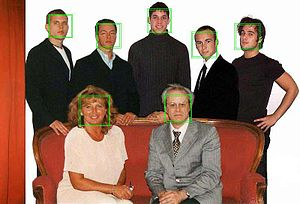
\includegraphics[scale=1]{cv-ejemplo.jpg}}
	\end{figure}
	La visión por computadora ha tenido un gran avance durante los últimos años debido, principalmente, a las mejoras en hardware. Somos ahora capaces de realizar
	una mayor cantidad de cálculos en una cantidad mayor de datos gracias a un significativo aumento de la capacidad de cómputo. Estos progresos permiten 
	que se investigue y profundice más en este campo.

	Con la llegada de las redes neuronales se ha hecho posible la realización de tareas complejas como la clasificación de imágenes,
	la detección de objetos o la segmentación. Las redes de neuronas convolucionales se han convertido en el estándar para este campo
	de la ciencia. Estas son capaces de ver patrones visuales que a un humano, se le harían complicados, si no imposibles, de ver.

	\section{Redes de neuronas convolucionales}
	Las redes neuronales están compuestas por diferentes capas, que a su vez están compuestas por diferentes neuronas. Todas las redes
	tienen una capa de entrada, una o más capas intermedias y una capa de salida. Los nodos de las capas están conectados entre sí
	y estos pueden activar o no, dependiendo del resultado de su función asociada, el nodo al que están conectados. 
	\begin{figure}[H]
		\ffigbox[\FBwidth]
		{\caption[Red de Neuronas]{Red de Neuronas \cite{red}}}
		{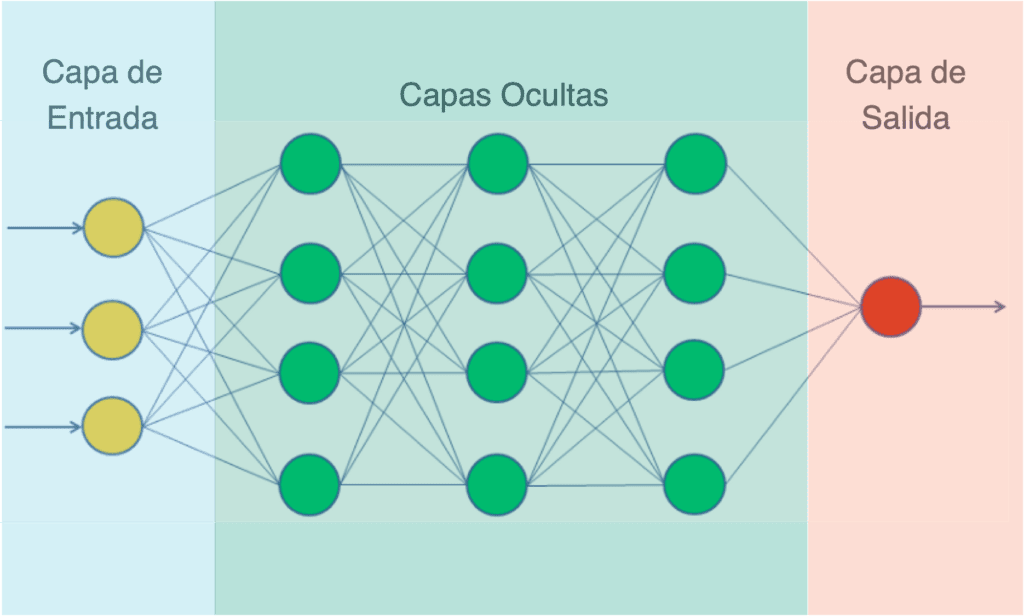
\includegraphics[scale=0.4]{red-neuronal.png}}
	\end{figure}
	Las redes de neuronas convolucionales son las que se utilizan para tareas de visión por computadora. Estas redes son mucho más eficientes
	a la hora de tratar con imágenes y esta es la razón por la que se usan en este campo del aprendizaje automático. En las primeras capas
	se identifican los elementos de la imagen a una escala grande, como pueden ser los bordes o los colores. A medida que se va profundizando
	en la red se van reconociendo partes más grandes de la imagen. Una vez se llega al final, la red es capaz de identificar el tipo de imagen. 
	Las redes convolucionales se componen de tres capas:
	\begin{itemize}
		\item \textbf{Capa convolucional:} en esta capa se aplica el proceso conocido como convolución. Se aplica un filtro (kernel)
		con el fin de detectar las características que se buscan en la imagen. 
		\item \textbf{Capa de agrupación:} en esta capa se aplica una reducción de dimensionalidad. Esta capa es muy importante ya que, aunque se
		pierde en  información, se gana en eficiencia.
		\item \textbf{Capa totalmente conectada:} en esta capa, a diferencia de las demás, todos los nodos están conectados a algún nodo
		de la capa anterior. 
	\end{itemize}
	Existen varios tipos de redes de neuronas convolucionales, entre ellas: AlexNet \cite{alexNet}, GoogleNet \cite{googleNet}, 
	ResNet \cite{resNet}, ZFNet \cite{zfnet} o VGGNet \cite{vgg16-paper}.
	Para la realización de este proyecto se ha optado por usar la última.

	\section{Extracción de características}
	Para la extracción de características se ha optado por usar la arquitectura VGG16. Esta arquitectura fue propuesta por
	Karen Simonyan y Andrew Zisserman en el artículo ``VERY DEEP CONVOLUTIONAL NETWORKS FOR LARGE-SCALE IMAGE RECOGNITION'' \cite{vgg16-paper}.
	\begin{figure}[H]
		\ffigbox[\FBwidth]
		{\caption[Estructura VGG16]{Estructura VGG16 \cite{art-vgg}}}
		{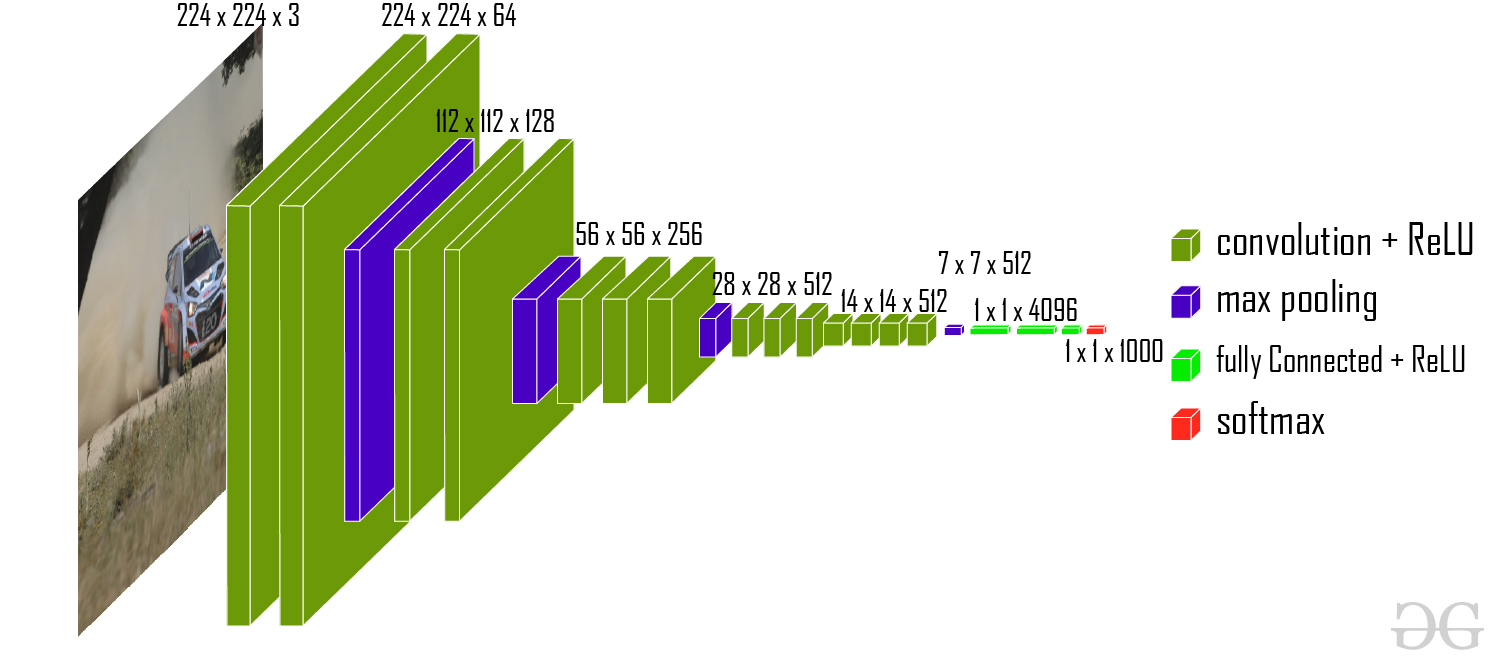
\includegraphics[scale=0.3]{vgg-funcionamiento.jpg}}
	\end{figure}

	Este modelo consiguió un 92,7\% de aciertos en el set de datos ``ImageNet'' \cite{imageNet}, que contiene más de catorce millones de imágenes.
	Es uno de los modelos más populares a la hora de trabajar con la extracción de características en imágenes. Es muy útil para
	conseguir clasificar imagénes, o en el caso de este proyecto, para calcular similitud entre ellas.

	La arquitectura VGG16 se ha elegido por varias razones. En primer lugar, esta está ampliamente documentada y es fácilmente accesible
	a través de bibliotecas de \textit{Python}. Aún siendo una arquitectura más simple que las demás opciones está contrastada como
	un modelo con un gran rendimiento en tareas de visión artificial, lo que la convierte en una elección sólida para un sistema de recomendación
	de imágenes. Además, esta arquitectura probó ser la más eficaz en el artículo ``Image-based Product Recommendation System with Convolutional Neural
	Networks'' \cite{stanford-paper}.

	\section{Segmentación de imágenes}
	En cuanto a la segmentación de imágenes se refiere destaca U2-Net, que es la arquitectura que se ha elegido.
	Presentada por investigadores de la universidad de Canadá en el año 2020, esta arquitectura se ha expandido
	rápidamente en el ámbito de la visión artificial debido a su gran eficacia.

	U2-Net consigue una sementación muy precisa haciendo uso de capas convolucionales y deconvolucionales, llegando de esta manera
	a captar caracacterterísticas a un nivel profundo. Tiene una gran capacidad para conservar algunos de los detalles más pequeños,
	lo que lo hace ideal para la segmentación de imágenes de moda. 


	U2-Net es una arquitectura líder en cuanto a la segmentación de imágenes. Además su uso resulta fácil en \textit{Python}, y
	por estas razones se ha optado por hacer uso de ella.


	\section{Trabajos similares}
	Hay muchos trabajos previos similares a este. Entre ellos destacan:
	\begin{itemize}
		\item ``Image-based Product Recommendation System with Convolutional Neural
		Networks'' \cite{stanford-paper}. En este artículo se describen las técnicas utilizadas para realizar un sistema de recomendación
		para tiendas online basado en la similitud entre imágenes. Se prueban los algoritimos SVG, AlexNet y VGG. Tras evaluar los tres
		este último resulta ser el más preciso. Una vez obtenidos los vectores de las imágenes se calcula la distancia coseno entre estos
		para calcular la similitud entre ambas. Este trabajo se relaciona fácilmente con el propuesto, ya que resuelve el problema haciendo uso del mismo
		modelo de clasificación y el mismo algoritmo de recomendación.
		\item ``Image-Based Service Recommendation System: A JPEG-Coefficient RFs Approach'' \cite{image-based-paper}. 
		Este artículo consta de dos fases. En la primera tratan de clasificar las imágenes según el tipo de producto mientras 
		que en la segunda se crea un sistema de recomendación que trata de encontrar los productos más similares a otro dado. 
		Para la segunda fase, que es la que aplica en nuestro caso, se usan coeficientes JPEG para sacar las 
		características de las imágenes. Después se calcula la distancia euclidiana entre estas. Este otro trabajo propone una
		manera diferente de resolver el objetivo a la utilizada en nuestro caso.
	\end{itemize}

	Este trabajo se diferencia en varios aspectos de los anteriores. En primer lugar, se añade el uso de máscaras para obtener recomendaciones
	que no se vean influenciadas por factores ajenos a la prenda en sí. Además, no solo se busca una recomendación en base a una imagen inicial,
	si no que también se permite al usuario seleccionar los atributos que quiere que tengan las imágenes recomendadas. A esta principal diferencia
	se suma el hecho de que este proyecto no se queda solo en un modelo, también
	cuenta con una interfaz gráfica que permite a los usuarios hacer uso de este. Este trbajo hace uso de arquitecturas de redes convolucionales ya existentes
	y combina métodos ya explorados para crear un sistema de recomendación, pero no propone ningún avance desde el punto de vista de estas arquitecturas.

	\chapter{Diseño del sistema}
	Este apartado pretende abordar el diseño del sistema, detallando como las distintas partes de este funcionan y trabajan en conjunto para
	resolver el problema propuesto. En primer lugar se describe el conjunto de datos empleado y posteriormente el modelo de inteligencia artificial.
	Después, la API y como esta sirve para comunicar el modelo con la interfaz gráfica. Esta última se presenta a través de imágenes. Finalmente, se procede
	a enumerar todas las tecnologías empleadas.
	\section{Conjunto de datos}
	Como se mencionó en el apartado ``Marco Reguador'' en este trabajo se hace uso del conjunto de datos 
	``iMaterialist (Fashion) 2020 at FGVC7'' \cite{imaterialist}. Este conjunto de datos cuenta con varios archivos que se 
	explican a continuación.

	En primer lugar tenemos dos conjuntos de imágenes, ``train'' y ``test''. El conjunto ``train'' cuenta con 43.793 imágenes
	y ``test'' con 3200. Ambos conjuntos contienen estas imágenes nombradas por un identificador.
	\begin{figure}[H]
		\ffigbox[\FBwidth]
		{\caption{Ejemplo de imagen en el conjunto de datos}}
		{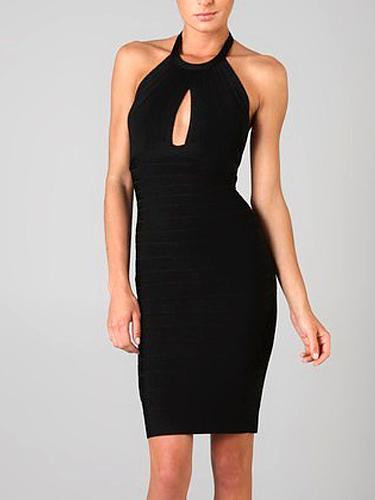
\includegraphics[scale=0.4]{ejemplo-dataset.jpg}}
	\end{figure}

	Además hay un archivo llamado ``train.csv'' que contiene los siguientes campos:
	\begin{itemize}
		\item \textbf{imageId}: identificador único para las imágenes. Para cada imagen hay varias entradas en el archivo, tantas como segmentaciones
		tenga la imagen
		\item \textbf{encodedPixels}: estos pixeles son la segmentación de la imagen
		\item \textbf{height}: altura de la imagen
		\item \textbf{width}: ancho de la imagen
		\item \textbf{classId}: identificador de la clase a la que pertenecen
		\item \textbf{attributesIds}: lista de identificadores de atributos que contiene este segmento de la imagen 
	\end{itemize}

	La segmentación es de gran utilidad, ya que sirve para realizar las máscaras de las imágenes. 
	También se destaca el campo \textbf{attributesIds} ya que gracias a este podemos filtrar las 
	imágenes a gusto del usuario. Estos atributos vienen descritos en un archivo llamado ``label\textunderscore descriptions.json''.
	Cada atributo tiene una descripción y una supercategoria asociadas a su identificador único.

	\section{Modelo}
	\subsection{Segmentación}
	En primer lugar se deben preprocesar las imágenes, el objetivo del trabajo es hacer recomendaciones de prendas similares, por lo tanto
	todo lo que no sea una prenda en la imagen puede influir negativamente en la recomendación. Por ejemplo, se podrían recomendar prendas
	con el fondo de la imagen similar, imágenes que tengan una misma marca de agua o imágenes en las que los modelos que las visten tengan
	parecidos físicos, entre otras cosas.
	Estos aspectos no deberían influir en la recomendacion por lo que lo primero que se realiza son las máscaras de las imágenes. 
	Para ello se utiliza el atributo \textbf{encodedPixels}.
	Con estos pixeles, que son una segmentación de las prendas, se puede obtener una imagen que consista únicamente en ropa.
	A continuación se muestra un ejemplo de una imagen antes y después de aplicarle la máscara.
	\begin{figure}[H]
		\centering
		\begin{subfigure}{0.4\textwidth}
			\centering
			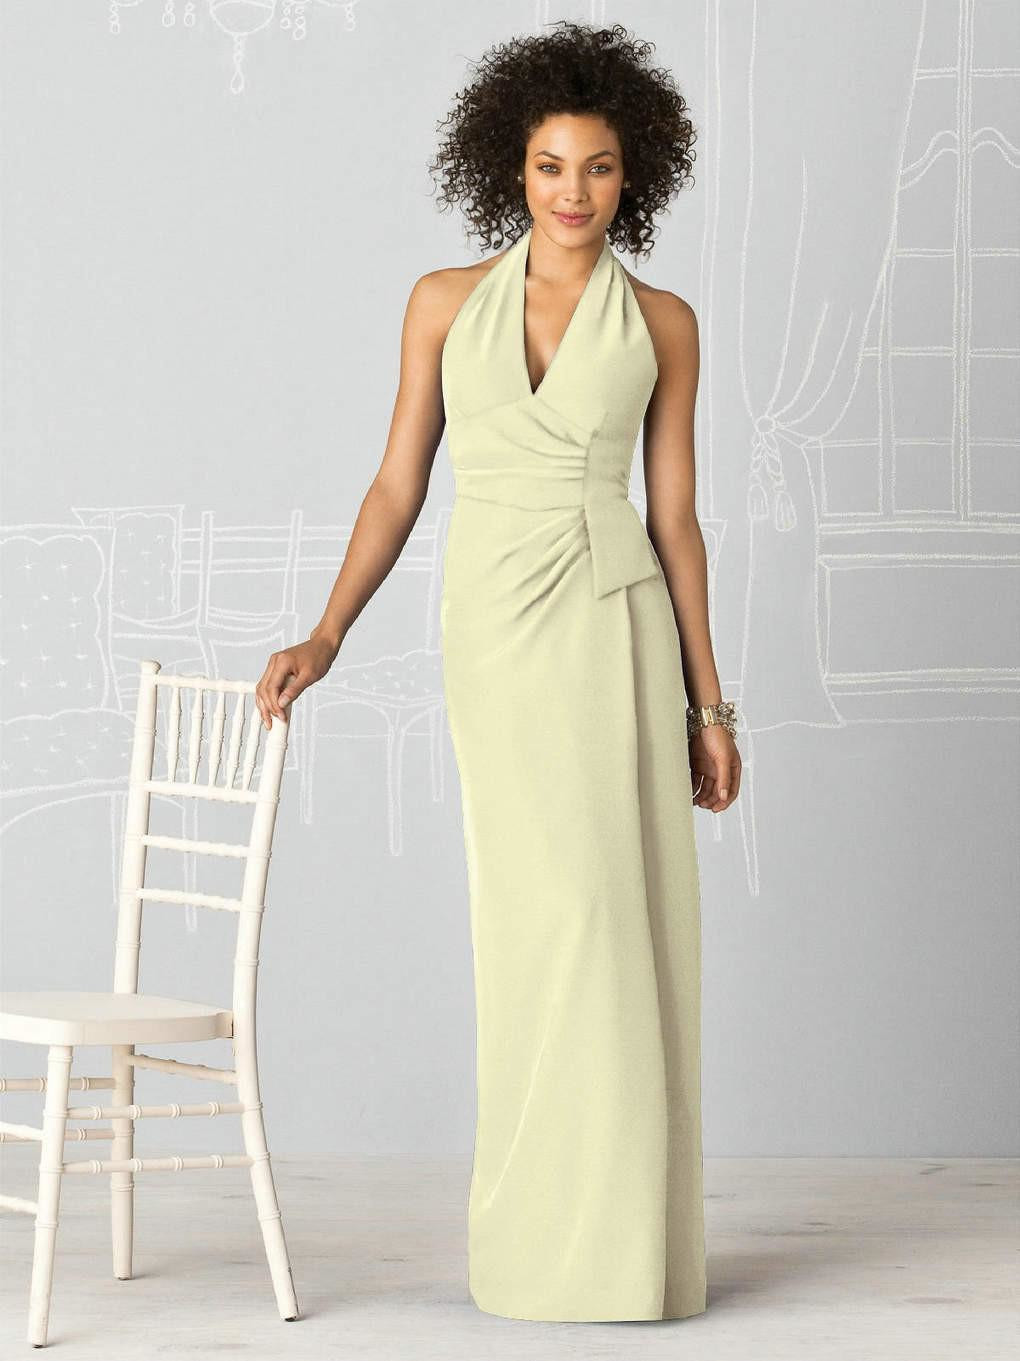
\includegraphics[width=\linewidth]{ejemplo-sin-mascara.jpg}
		\end{subfigure}
		\begin{subfigure}{0.45\textwidth}
			\centering
			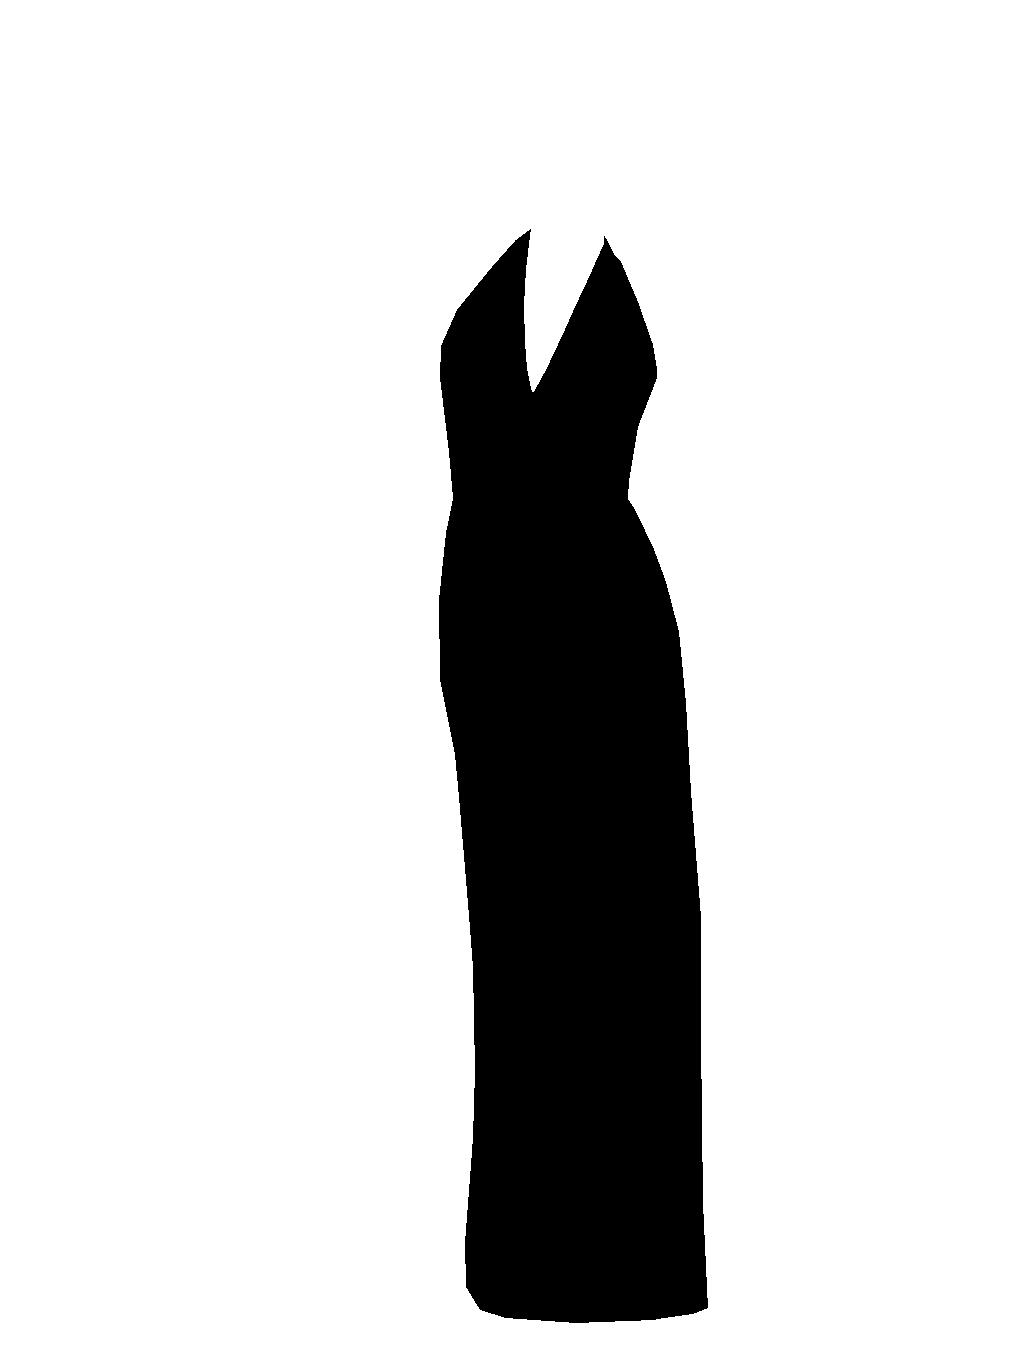
\includegraphics[width=\linewidth]{ejemplo-con-mascara.jpg}
		\end{subfigure}
		\caption{Ejemplo de imagen antes y después de aplicar la máscara}
	\end{figure}

	Como se puede observar en la figura, la máscara ha quitado todo excepto la prenda.
	Todas estas máscaras son pre-procesadas y almacenadas, ya que serán las que se usen para el modelo.


	Esto no es suficiente, ya que el usuario proporciona una imagen que no está en la base de datos, por lo que no se tiene la segmentación de esta.
	Debido a este motivo es necesario hacer uso de un modelo de segmentación para generar la máscara de la imagen dada por el usuario.
	Hay un gran número de arquitecturas que podrían resolver este problema. A continuación se describen algunas de ellas:
	\begin{itemize}
		\item \textbf{U-Net \cite{unet}:} su nombre viene dado porque su arquitectura tiene forma de U, combina capas de convolución y deconvolución para conseguir la segmentación de las imágenes.
		\item \textbf{SegNet \cite{segNet}:} utiliza capas de \textbf{pooling} para conseguir el objetivo de segmentar las imágenes.
		\item \textbf{Mask R-CNN \cite{rcnn}:} esta arquitectura es una combinación de \textbf{Faster R-CNN}, que sirve para la detección de objetos, con la generación de máscaras.
		\item \textbf{DeepLab \cite{deeplab}:} esta arquitectura utiliza la convolución dilatada para lograr el objetivo de segmentar las imágenes.
		\item \textbf{U2-Net \cite{u2net}:} esta arquitectura es una extensión de \textbf{U-Net} que incluye mejoras sustanciales, mejora la precisión y el rendimiento.
	\end{itemize}


	Finalmente se elige hacer uso de la arquitectura \textbf{U2-Net}, que cuenta con todas las ventajas de \textbf{U-Net} pero teniendo una mayor precisión 
	y rendimiento. La precisión es aún mayor cuando actúa sobre imágenes de alta resolución,
	lo que la convierte en una gran candidata para la segmentación de imágenes de moda.

	\textbf{U2-Net} nació en el año 2020 en la universidad de Alberta, Canadá, con
	el artículo ``U2-Net: Going Deeper with Nested U-Structure for Salient Object Detection'' \cite{u2net}. Este artículo fue galardonado
	en 2020 como el mejor en reconocimiento de patrones.
	\begin{figure}[H]
		\ffigbox[\FBwidth]
		{\caption[Arquitectura U2-Net]{Arquitectura U2-Net \cite{u2net-gh}}}
		{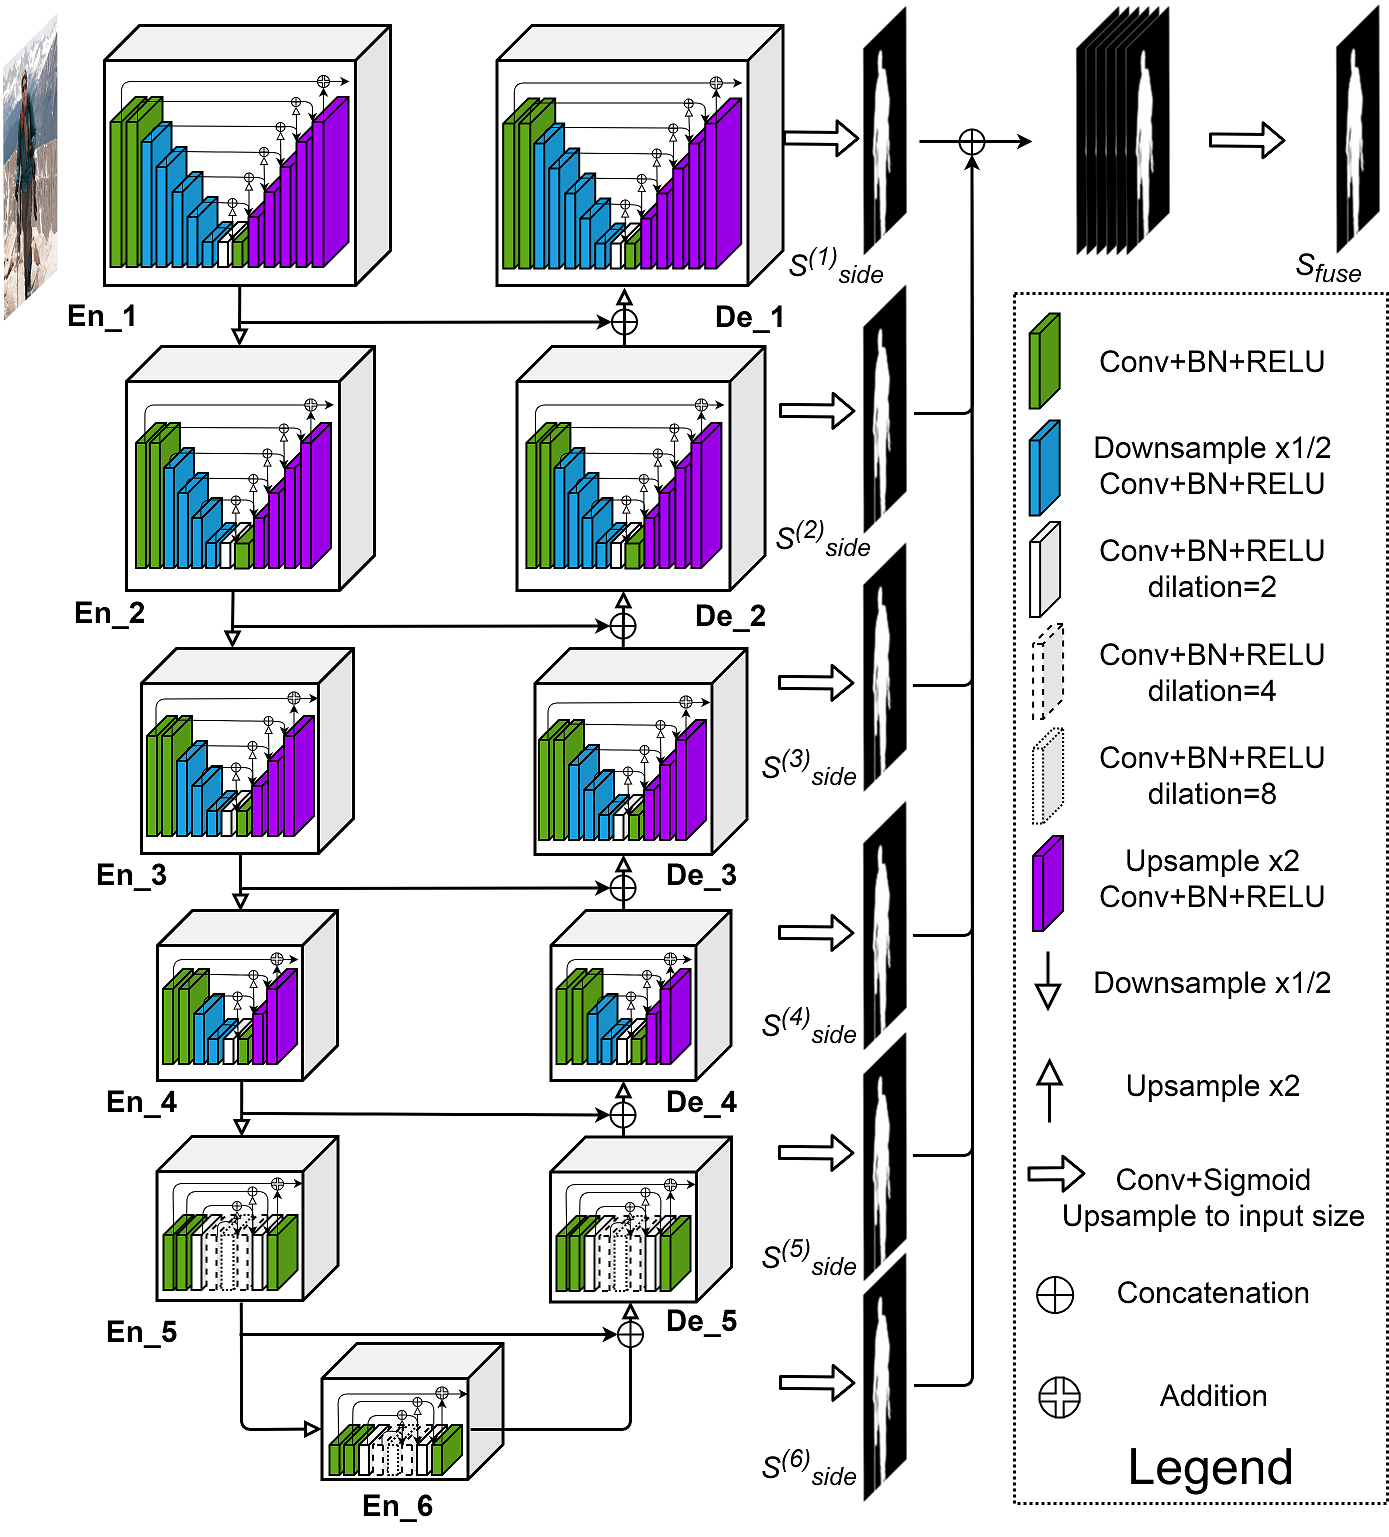
\includegraphics[scale=0.4]{u2net.png}}
	\end{figure}
	\begin{figure}[H]
		\ffigbox[\FBwidth]
		{\caption[Ejemplo de creación de máscaras con la arquitectura U2-Net]{Ejemplo de creación de máscaras con la arquitectura U2-Net \cite{u2net-gh}}}
		{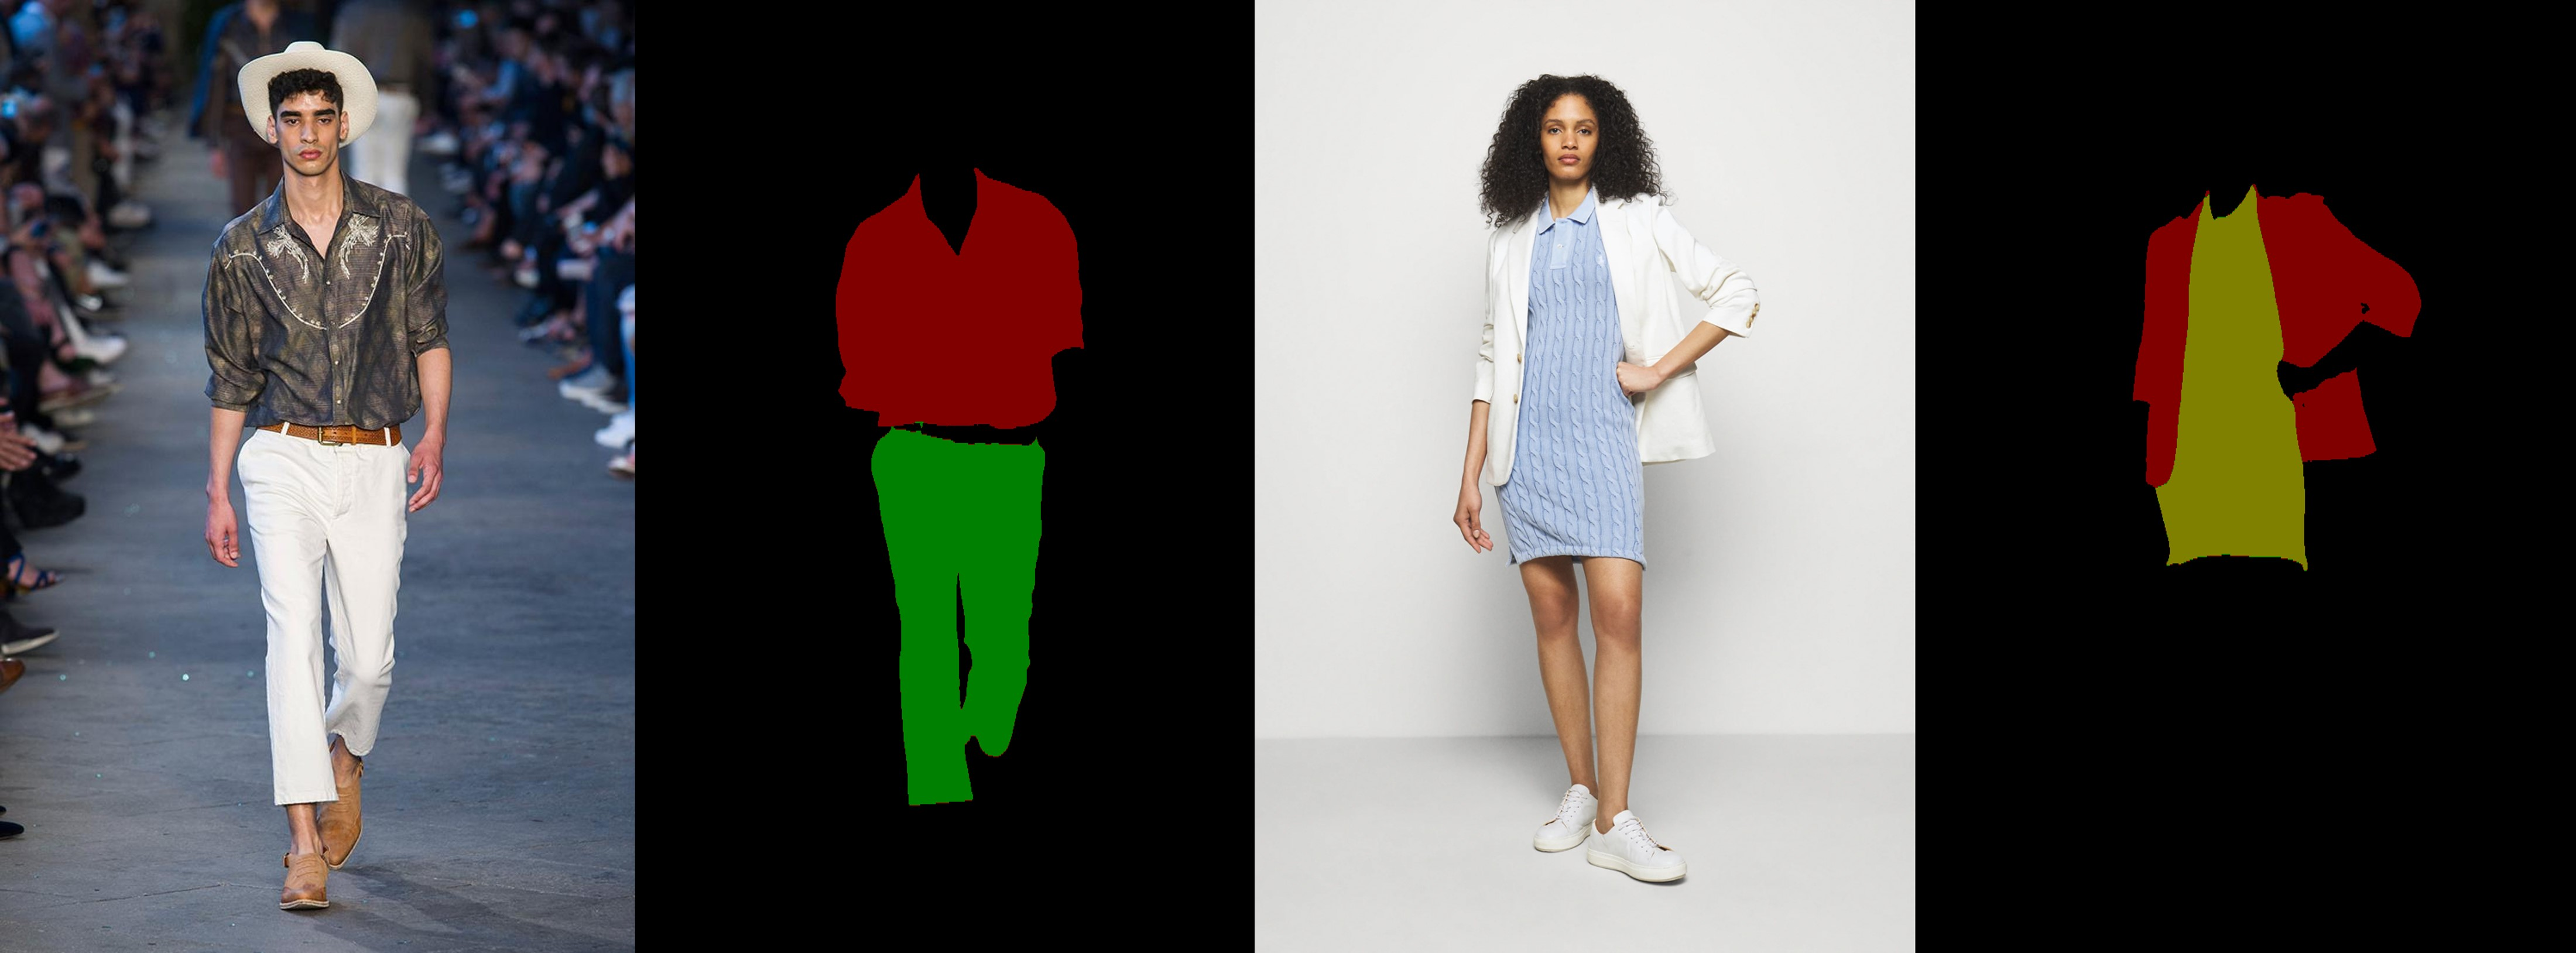
\includegraphics[scale=0.4]{u2net-mascara.jpg}}
	\end{figure}

	\subsection{Algoritmo de recomendación}
	El siguiente paso es extraer las características de todas las imágenes. Para ello se hace uso de
	una red de neuronas convolucional. Como ya se mencionó anteriormente se ha optado por 
	elegir el modelo VGG16. Este modelo tiene una estructura fácil de entender y es un modelo más profundo
	que sus predecesores, como puede ser AlexNet, lo que permite extraer características de mayor complejidad.
	\begin{figure}[H]
		\ffigbox[\FBwidth]
		{\caption[Estructura algoritmo VGG16]{Estructura algoritmo VGG16 \cite{vgg}}}
		{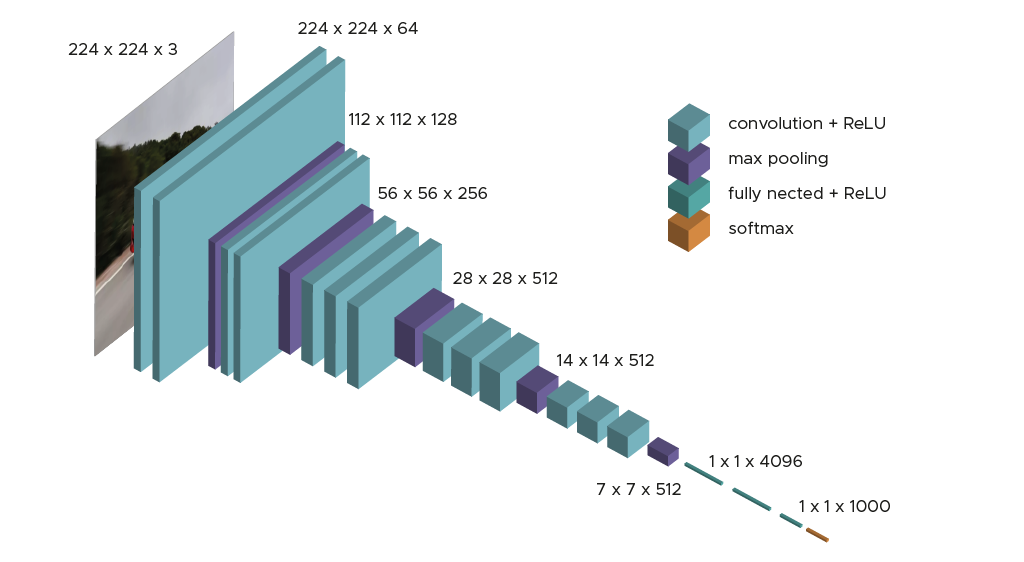
\includegraphics[scale=0.4]{vgg16.png}}
	\end{figure}

	El modelo hace uso de la arquitectura VGG16 y extrae el vector de características de todas las máscaras.
	Estos vectores son almacenados en una matriz. Cuando el usuario proporciona una imagen, se genera su máscara con el procedimiento
	mencionado anteriormente. Después se obtiene también su vector de características y se calcula la similitud coseno
	con los vectores de todas las demás imágenes. Finalmente se filtra el conjunto de datos por las prendas
	que contengan los atributos seleccionados por el usuario y se devuelven las $N$ imágenes con la mayor similitud,
	donde $N$ es el número de imágenes que el usuario desea obtener.
	El siguiente diagrama resume el funcionamiento del modelo.

	\begin{figure}[H]
		\ffigbox[\FBwidth]
		{\caption{Diagrama del funcionamiento del modelo}}
		{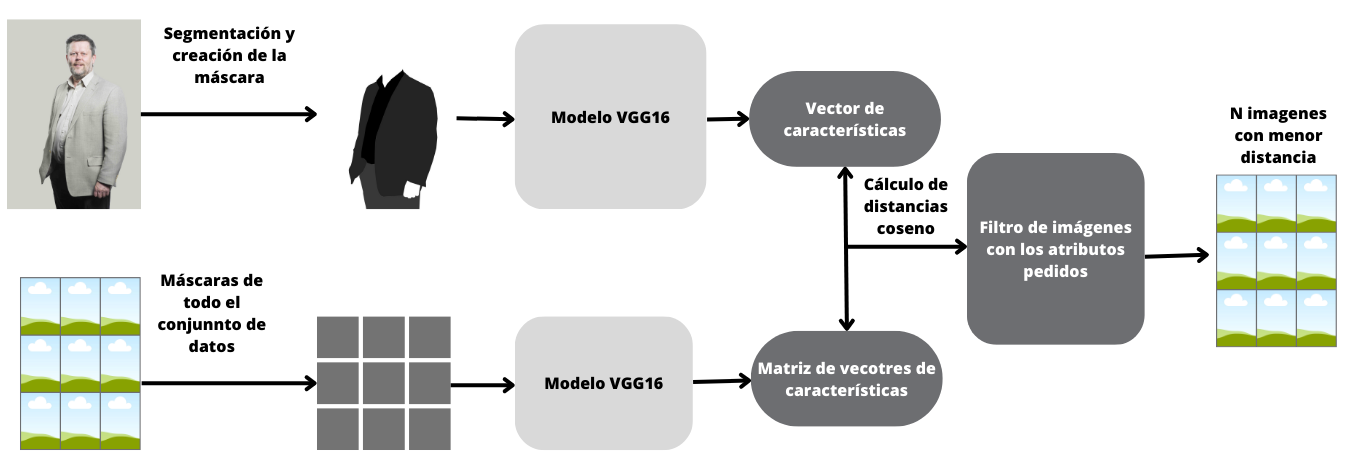
\includegraphics[scale=0.45]{diagrama-modelo.png}}
	\end{figure}

	\section{API}
	Con el fin de poder crear una interfaz gráfica fácil de usar para un usuario común es necesario tener una API que sirva el modelo.
	Una API es una forma de conectar diferentes aplicaciones para lograr que trabajen juntas. La API permite
	a la interfaz gráfica poder consumir el modelo de inteligencia artificial.

	Se ha optado por hacer esta API en \textit{Python}, ya que facilita el desarrollo al estar el modelo también hecho con
	este mismo lenguaje. La librería elegida para construir esta API es Flask, un \textit{framework} diseñado para poder hacer
	aplicaciones CRUD (\textit{Create}, \textit{Read}, \textit{Update}, \textit{Delete}). Una aplicación CRUD puede tener varios
	\textit{endpoint}, rutas a las que enviar una solicitud. Cada una de estas rutas puede realizar las acciones 
	de crear, leer, actualizar o borrar información en la API.
	
	En el caso de nuestra API solo han sido necesarios dos \textit{endpoints}.

	\begin{itemize}
		\item \textbf{``/recommendations'':}
		
		Usa el método \textit{POST}. Este \textit{endpoint} espera
		recibir una imagen, un número de recomendaciones y una lista de identificadores de atributos opcional. Una vez
		recibe estos argumentos, la API hace uso del modelo y devuelve la lista de identificadores de las imágenes que,
		teniendo los atributos requeridos, tengan la mayor similitud.
		\begin{figure}[H]
			\ffigbox[\FBwidth]
			{\caption{Ejemplo de peteción al \textit{endpoint} ``/recommendations''}}
			{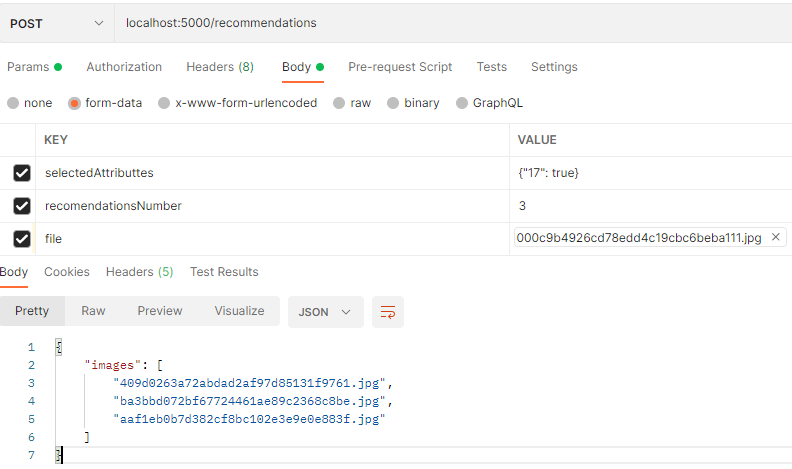
\includegraphics[scale=0.8]{postman-recommendations.png}}
		\end{figure}
		\item \textbf{``/image/<id>'':}
		
		La API permite recuperar imágenes a partir de su identificador gracias a este \textit{endpoint}, donde
		``id'' es el identificador de la imagen que se desea obtener. Solo es necesario hacer una petición de tipo \textit{GET}
		con un identificador válido en la ruta.
	
		\begin{figure}[H]
			\ffigbox[\FBwidth]
			{\caption{Ejemplo de peteción al \textit{endpoint} ``/image/<id>''}}
			{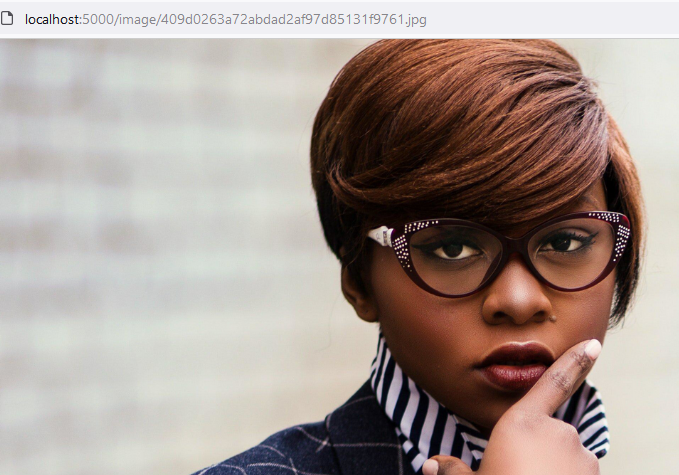
\includegraphics[scale=0.8]{ejemplo-peticion-imagen.png}}
		\end{figure}
	\end{itemize}

	\section{Interfaz}

	Para la interfaz gráfica se tuvieron en cuenta varias opciones. La primera de ellas fue \textit{StreamLit}, una plataforma
	para desarollorar interfaces para proyectos de inteligencia artificial escrita en \textit{Python}. Permite desplegar este
	tipo de aplicaciones de una manera muy sencilla, escribiendo muy pocas líneas de código. Por otro lado se pensó en usar
	\textit{Gradio}, una plataforma que funciona de una manera muy similar a \textit{StreamLit}. Ambas opciones son buenas
	pero al final se decidió hacer uso del \textit{framework} de desarrollo \textit{React}, del leanguaje \textit{JavaScript}.
	Aunque las dos primeras herramientas eran interesantes para conseguir un desarrollo rápido, las opciones de interfaz quedaban limitadas.

	El hecho de no poder hacer la interfaz completamente a mi gusto fue lo que me hizo decantarme por \textit{React}, con el cual
	se puede hacer una web completa, con todas sus características. Además se hace uso de \textit{TypeScript}, en lugar
	de \textit{JavaScript}, ya que ofrece una mayor solidez gracias a su tipado estático. Esto ayuda a no cometer errores difíciles de
	depurar durante el desarrollo, aunque a veces pueda resultar tedioso el hecho de tener que marcar todos los tipos. El hecho de utilizar
	\textit{React} resulta muy útil, ya que se puede organizar el código por componentes reutilizables en donde se junta el \textit{HTML}
	con el \textit{JavaScript}.

	El proyecto tiene la siguiente estructura:
	\begin{figure}[H]
		\ffigbox[\FBwidth]
		{\caption{Estructura del proyecto}}
		{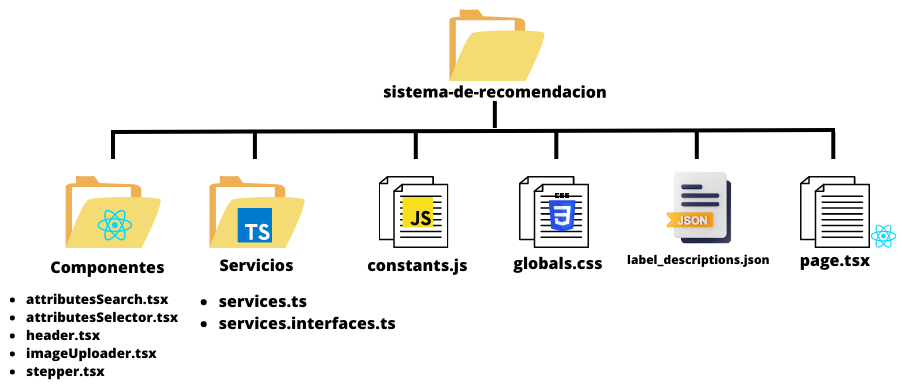
\includegraphics[scale=0.6]{estructura-carpetas.png}}
	\end{figure}

	\begin{itemize}
		\item \textbf{attributtesSearch.tsx}: este componente sirve para buscar los atributos que el usuario quiera
		seleccionar para que aparezcan en sus recomendaciones. Cuenta con la lista completa de atributos (que son elementos
		seleccionables) y con un buscador, ya que hay 341 atributos diferentes.
		\item \textbf{attributtesSelector.tsx}: este componente contiene la búsqueda de atributos. 
		Además cuenta con un botón para que, en caso de que el usuario así lo desee, 
		sirve para obtener recomendaciones de prendas con todo tipo de atributos.
		\begin{figure}[H]
			\ffigbox[\FBwidth]
			{\caption{Componente \textbf{attributesSearch}}}
			{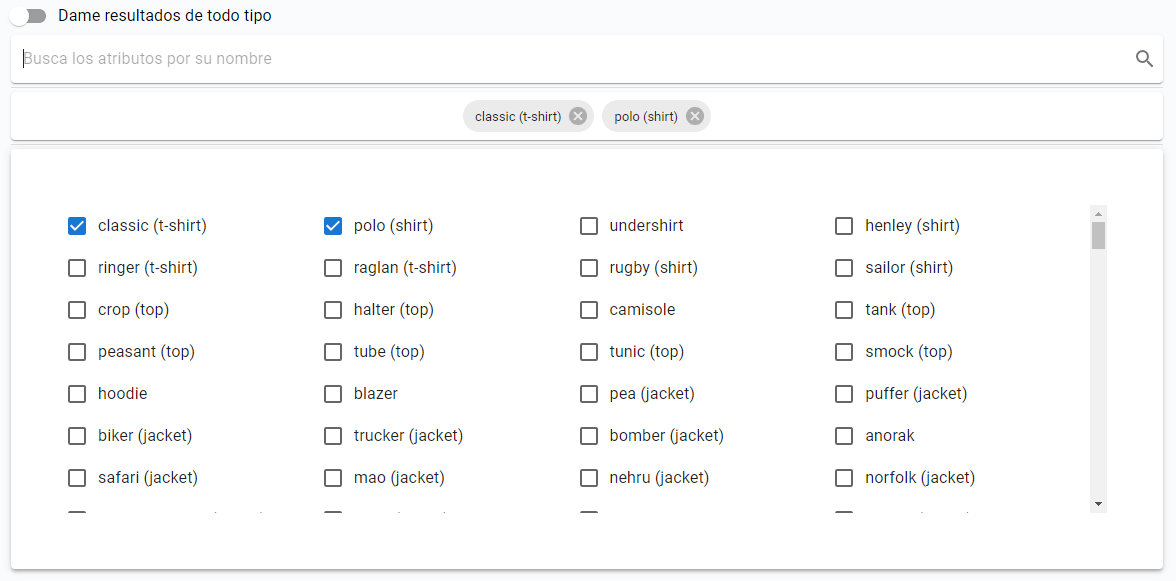
\includegraphics[scale=0.4]{attributes-search.png}}
		\end{figure}
		\item \textbf{header.tsx}: este es el encabezado de la página.
		\begin{figure}[H]
			\ffigbox[\FBwidth]
			{\caption{Componente \textbf{header}}}
			{
\includegraphics[scale=0.3]{header.png}}
		\end{figure}
		\item \textbf{imageUploader}: este componente es una caja que permite al usuario subir la imagen que
		desea utilizar para obtener recomendaciones. Esta permite explorar sus archivos locales y subir un
		archivo que debe ser de tipo imagen.
		\begin{figure}[H]
			\ffigbox[\FBwidth]
			{\caption{Componente \textbf{imageUploader}}}
			{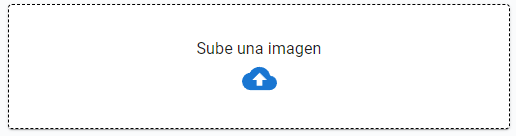
\includegraphics[scale=0.7]{image-uploader.png}}
		\end{figure}
		\item \textbf{stepper}: este componente sirve para pasar las pantallas del proceso de dar toda la información,
		ya que la aplicación consiste en una sola página.
		\item \textbf{services.ts}: este archivo se encarga de realizar las peticiones a la API.
		\item \textbf{services.interfaces.ts}: este archivo contiene las interfaces necesarias para los servicios.
		\item \textbf{constants.js}: en este fichero se almacenan las variables que son constantes a lo largo del proyecto.
		\item \textbf{globals.css}: en este fichero se guarda la configuración CSS que afecta a todo el proyecto.
		\item \textbf{label\textunderscore descriptions.json}: este archivo se usa para asociar los identificadores de los atributos
		a sus descripciones.
		\item \textbf{page.tsx}: esta es la página principal, donde todos los componentes se unen para componer la aplicación.
		

		Nada más cargar la página podemos ver una ventana que nos pide subir una imagen. Una vez subida la imagen
		se puede presionar el botón de ``siguiente'', el cual nos lleva a seleccionar el número de recomendaciones, 
		a través de una barra de selección de números. Una vez más es posible presionar el botón
		de ``siguiente'', esta vez nos llevará a la ventana final, la selección de atributos. Esta contiene la lista completa de los 
		atributos seleccionables. Los atributos seleccionados quedan marcados en la parte superior, desde donde se puede 
		eliminar la selección. Además hay un buscador dada el gran número de atributos que hay. Una vez ya está todo listo se
		puede pulsar sobre el botón ``procesar''. Este botón manda una petición a la API que, haciendo uso del modelo, devuelve los
		identificadores de las imágenes con mayor similitud. Con estos identificadores se vuelve a hacer una petición por cada uno de
		ellos para obtener sus respectivas imágenes. Estas imágenes se muestran en una galería que se puede poner a tamaño completo.
		Si se desea repetir el proceso basta con pulsar el botón ``resetear''.

		A continuación se muestra, a través de imágenes, el funcionamiento descrito anteriormente.
		\begin{figure}[H]
			\ffigbox[\FBwidth]
			{\caption{Pantalla inicial, subida de imagen}}
			{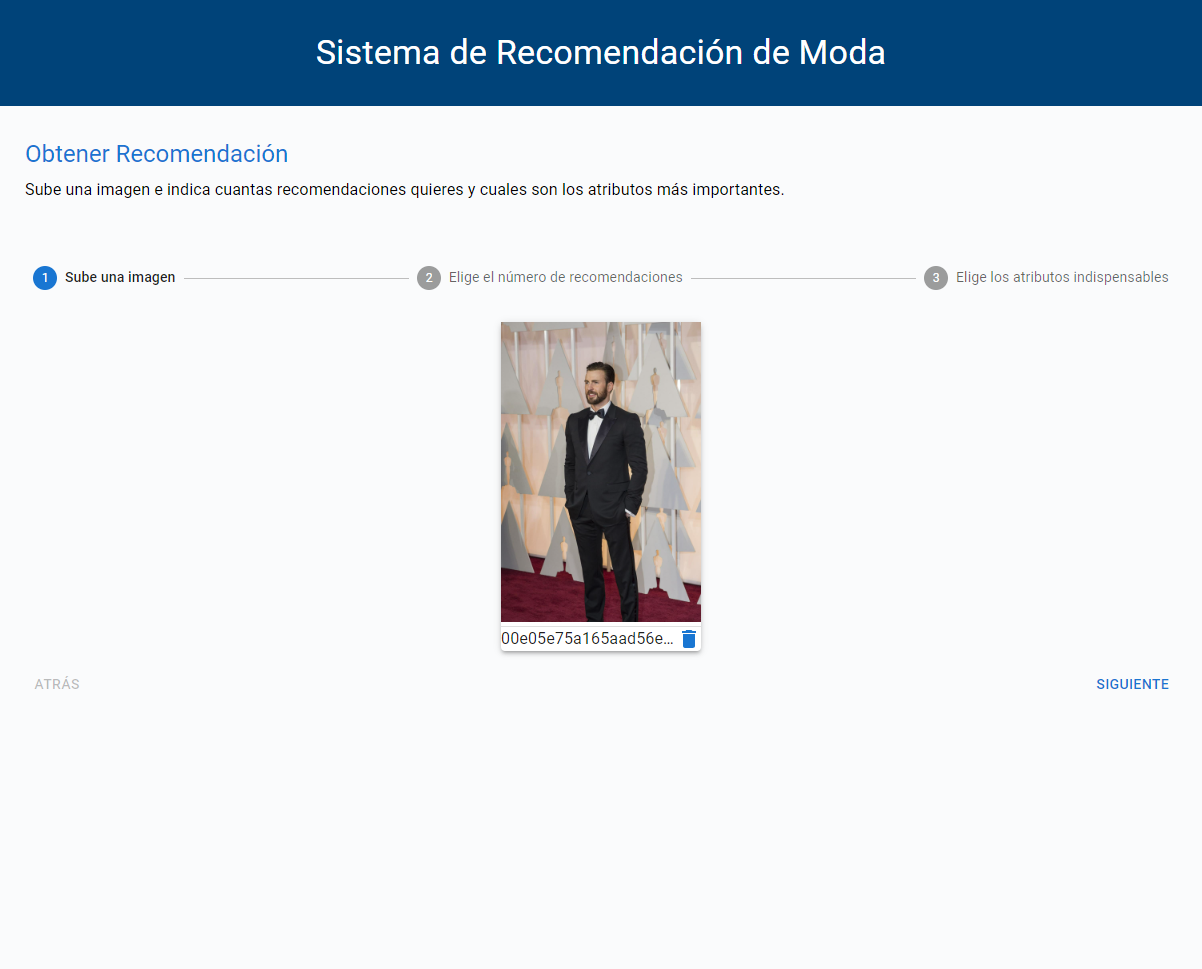
\includegraphics[scale=0.3]{pantalla-1.png}}
		\end{figure}
		\begin{figure}[H]
			\ffigbox[\FBwidth]
			{\caption{Selección del número de recomendaciones}}
			{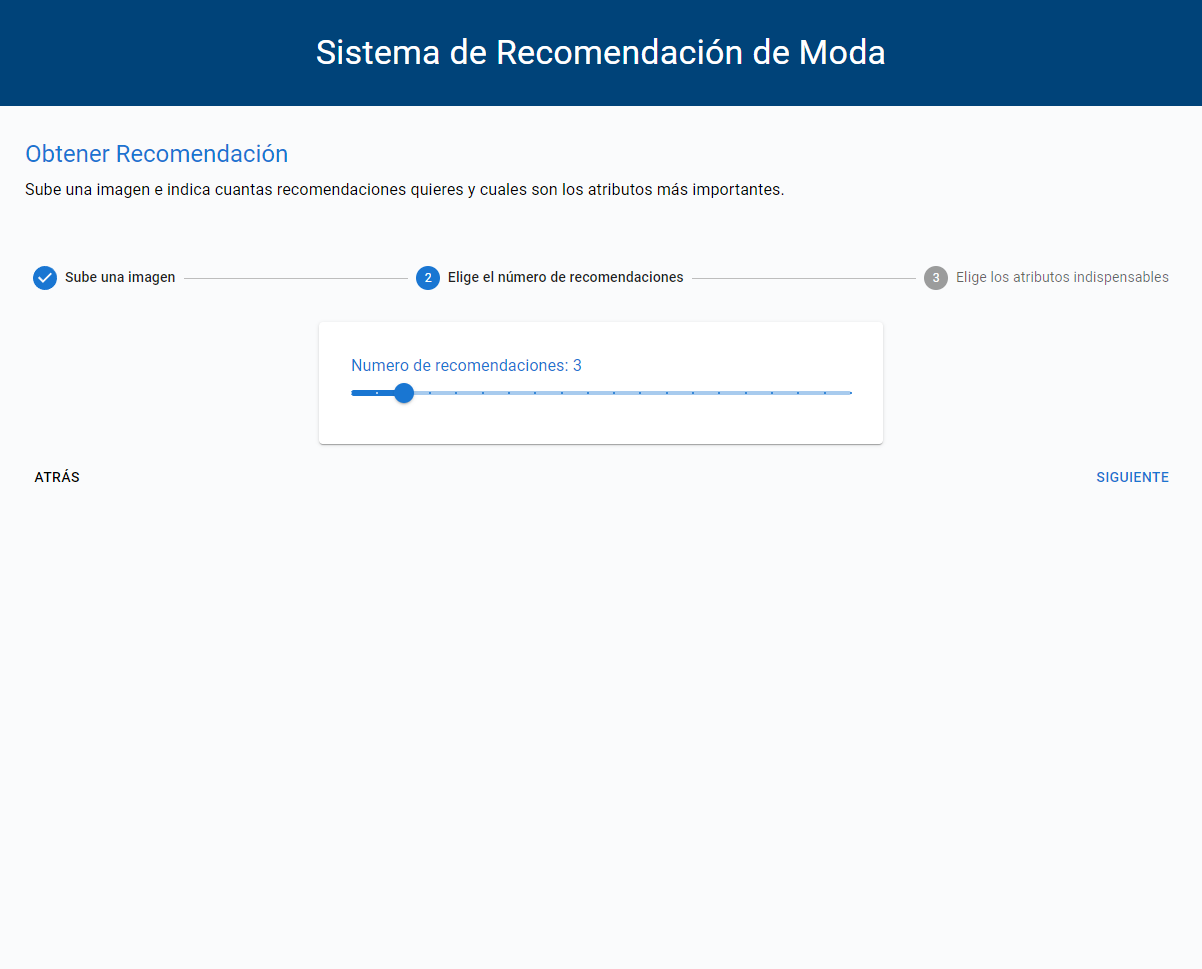
\includegraphics[scale=0.3]{pantalla-2.png}}
		\end{figure}
		\begin{figure}[H]
			\ffigbox[\FBwidth]
			{\caption{Selección de atributos}}
			{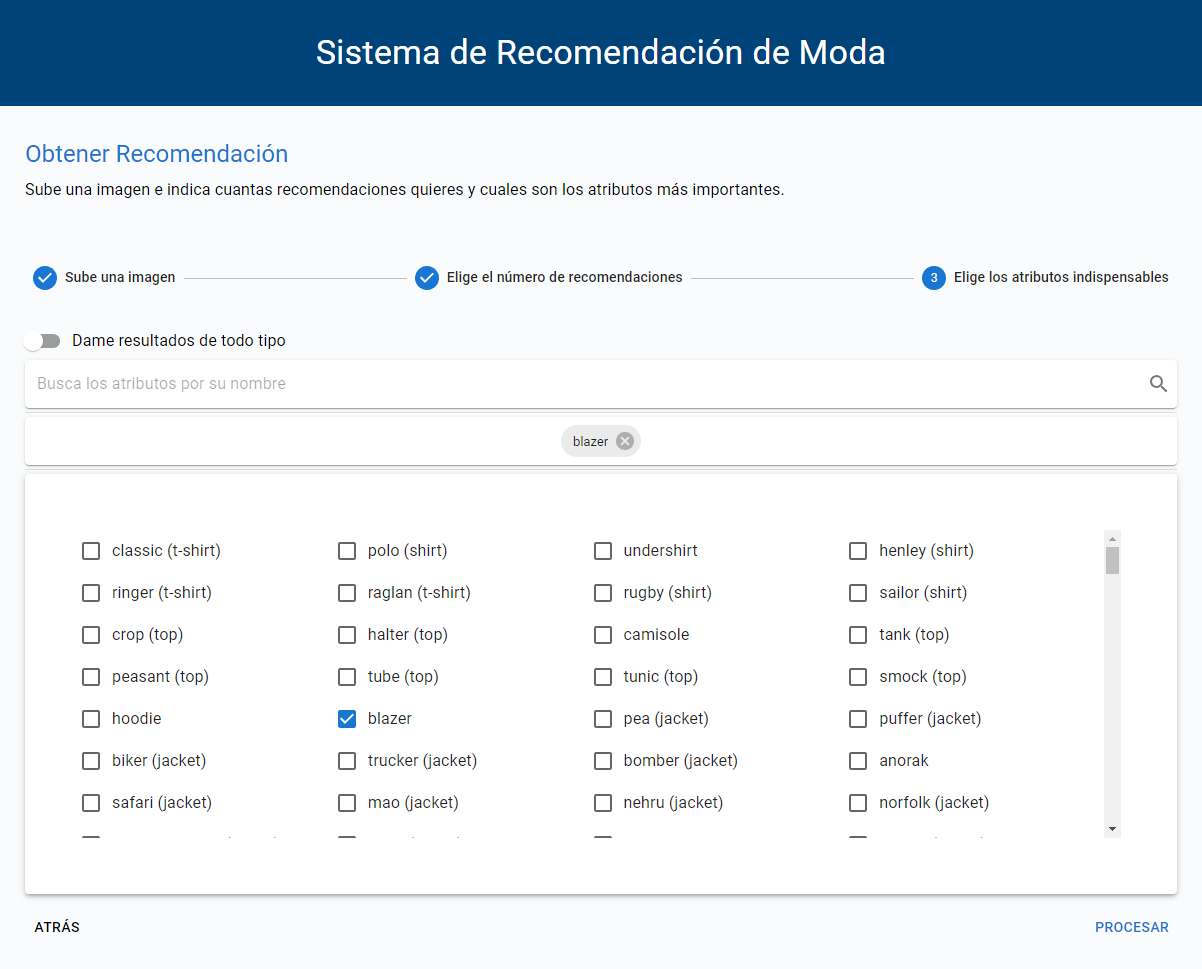
\includegraphics[scale=0.3]{pantalla-3.png}}
		\end{figure}
		
		\begin{figure}[H]
			\ffigbox[\FBwidth]
			{\caption{Barra de carga mientras la API procesa la solicitud}}
			{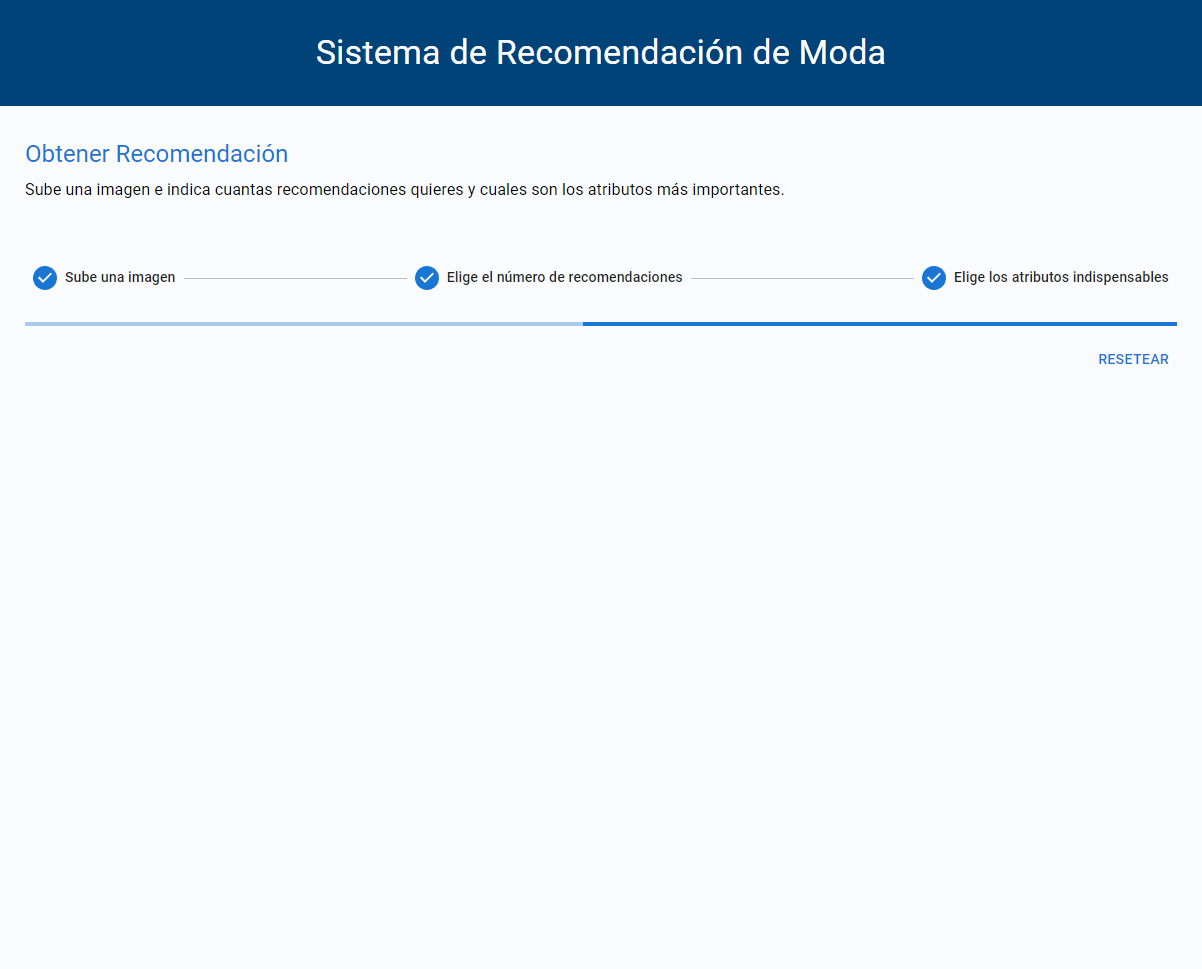
\includegraphics[scale=0.3]{pantalla-carga.png}}
		\end{figure}
		\begin{figure}[H]
			\ffigbox[\FBwidth]
			{\caption{Resultado del proceso. Recomendaciones.}}
			{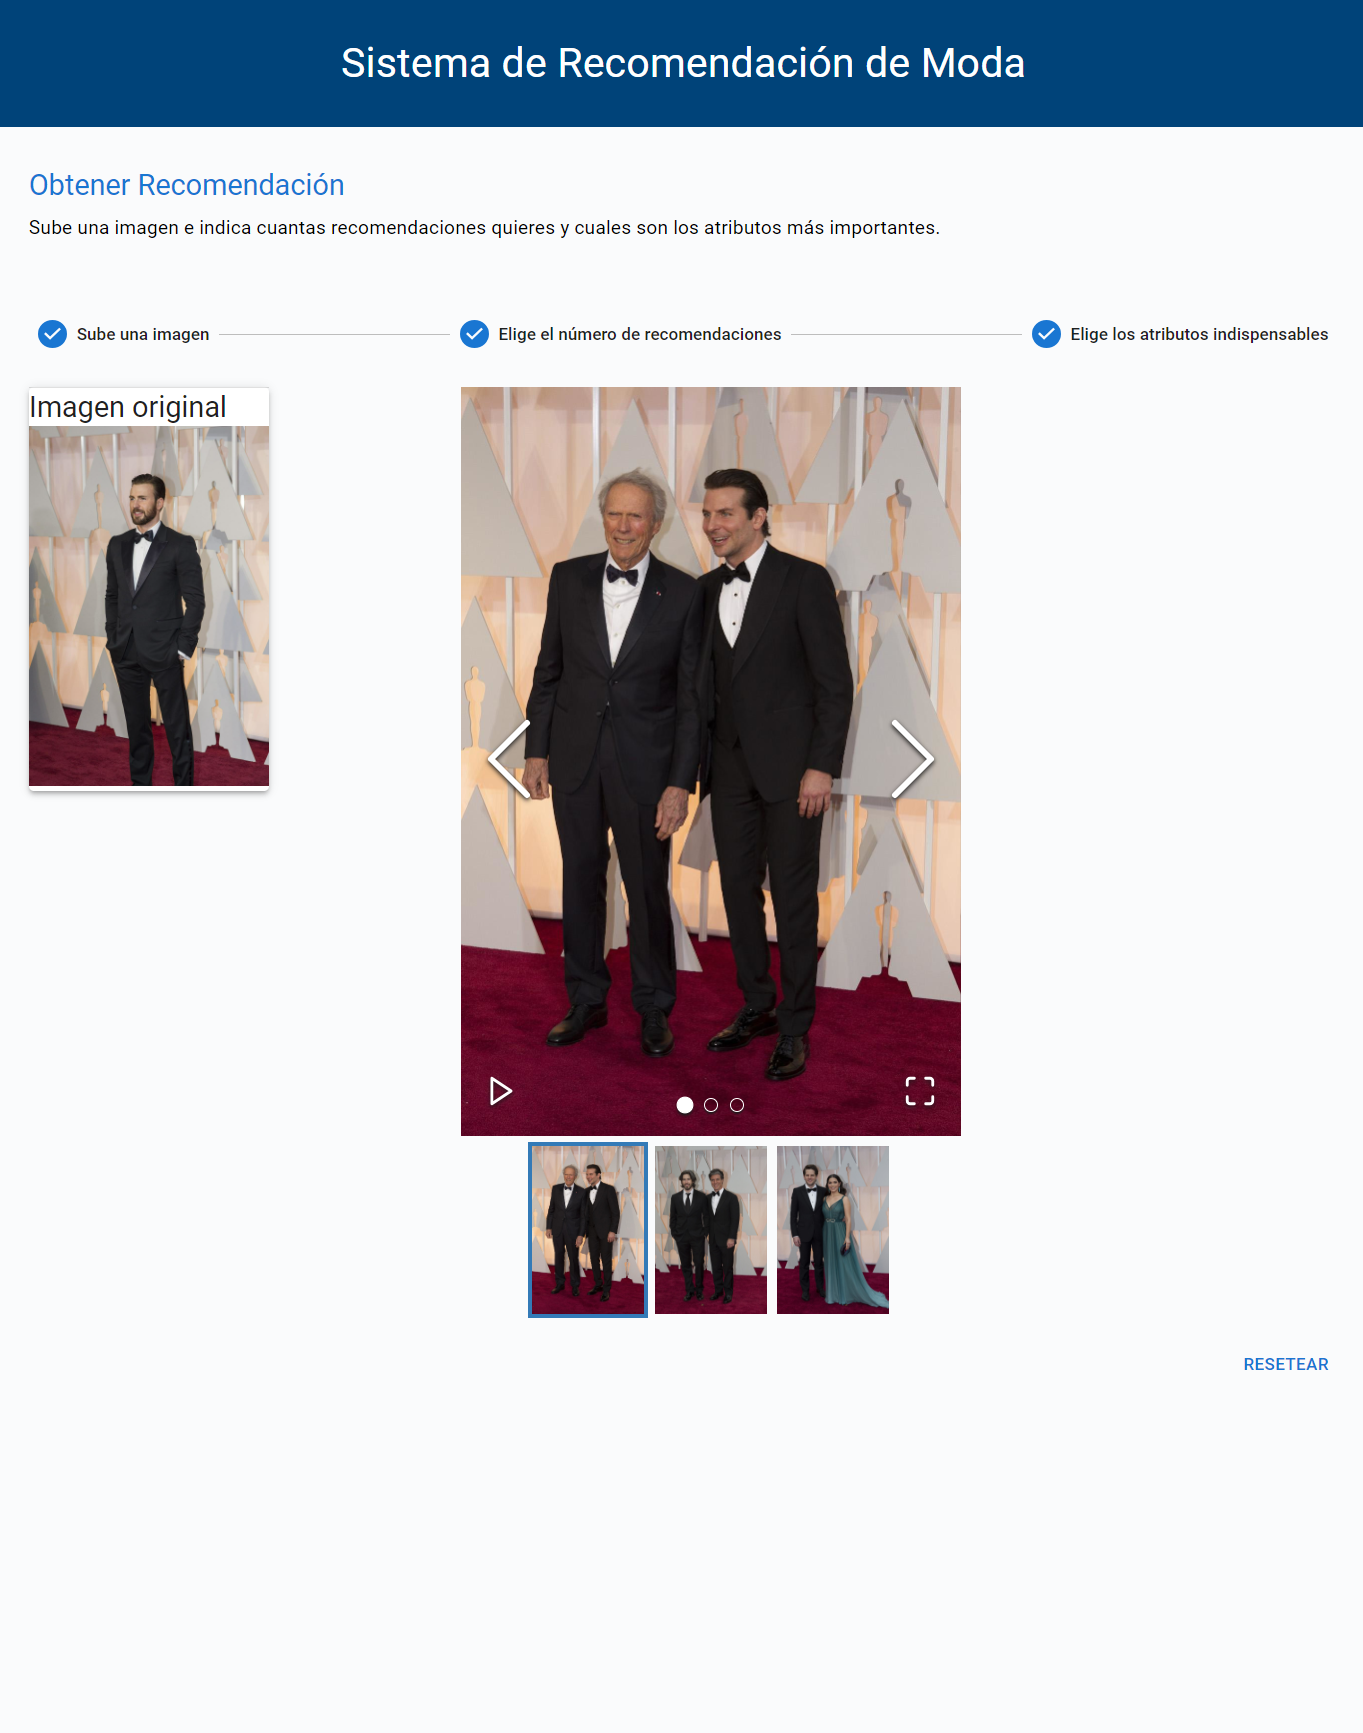
\includegraphics[scale=0.4]{output.png}}
		\end{figure}

	\end{itemize}

	\section{Tecnologías empleadas}
	Para la realización de este trabajo ha sido necesario el uso tanto de hardware como de software.
	En la siguiente tabla se muestra el hardware utilizado.
	\begin{table}[H]
		\centering
		\caption{Especificaciones del hardware utilizado}
		\begin{tabular}{llll}
				\toprule
				\textbf{Equipo} & \textbf{RAM} & \textbf{CPU} & \textbf{GPU}\\
				\midrule
				\textbf{Ordenador de sobremesa} & 16 GB & AMD RYZEN 53500X & AMD Radeon RX 5500 XT  \\
				\textbf{HP ENVY 13} & 8 GB & INTEL i7 & NVIDIA GeForce MX150 \\
				\bottomrule
		\end{tabular}
	\end{table}

	Ambos ordenadores tienen como sistema operativo \textit{Windows}, 10 y 11 respectivamente.
	Se ha hecho uso del IDE \textit{VScode}, de código abierto, para el desarrollo de tanto la API como la interfaz gráfica.
	
	
	En el caso de la API se ha usado el lenguaje de programación \textit{Python} junto con las siguientes librerías:
	
	\begin{itemize}
		\item \textbf{Flask}: \textit{framework} minimalista que sirve para desarrollar aplicaciones web. En este caso
		sirve para comunicar el modelo con la web. 
		\item \textbf{Pickle}: utilizada para cargar a memoria el modelo con la matriz de características extraídas de las imágenes.
		\item \textbf{OS}: utilizada para trabar con los archivos del sistema. Recuperar, crear y eliminar imágenes en él.
		\item \textbf{JSON}: manejo de objetos de tipo JSON. Utilizada para comunicarse con la aplicación web.
		\item \textbf{Numpy}: cálculos optimizados con las matrices que representan las imágenes. Utilización de algunas de sus
		funciones matemáticas. 
		\item \textbf{Keras}: utilizado para hacer uso de la arquitectura VGG16.  
		\item \textbf{Tensorflow}: utilizado para cargar imágenes y transformarlas a listas.
		\item \textbf{Scipy}: uso de su función optimizada para calcular la distancia coseno entre vectores, ya que ofrece un rendimiento
		superior y se reducen los tiempos de espera.
		\item \textbf{Pandas}: utilizado para usar la estructura \textit{Dataframe} que aporta una gran velocidad a la hora de trabajar
		con grandes cantidades de datos, como es el caso.
		\item \textbf{Matplotlib}: utilizado para generar gráficas que sirvieron para analizar el conjunto de datos.
	\end{itemize}

	La interfaz gráfica por otra parte ha sido desarrollada con \textit{TypeScript} junto con las siguientes librerías:
	\begin{itemize}
		\item \textbf{React}: este es el \textit{framework} principal utilizado en la interfaz gráfica. Aporta una gran facilidad para
		poder reutilizar código y no repetirlo. Además cuenta con multitud de librerías que resultan de gran utilizad.
		\item \textbf{Material UI}: librería para el \textit{framework React} que contiene elementos gráficos de UI. Además aporta
		una gran usabilidad a la web. 
		\item \textbf{Axios}: librería que sirve para realizar las peticiones web a la API.
		\item \textbf{React image gallery}: componente de \textit{React} que renderiza una galería de imágenes.
	\end{itemize}

	\chapter{Resultados}

	En este apartado se analizan los resultados obtenidos a través de ejemplos de entrada
	y salida. Además se comparan los resultados con y sin máscara y con y sin el uso de atributos.


	\section{Sin máscaras}

	En un inicio el sistema de recomendación funcionaba sin máscaras. Este sistema funcionaba correctamente pero
	tenía ciertas desventajas:
	\begin{itemize}
		\item En ocasiones la recomendación se fijaba en el color de fondo de las imágenes en lugar de las prendas en sí.
		\item Tenía en cuenta los modelos que vestían las prendas.
		\item Recomendaba prendas con el mismo color.
		\item Tenía en cuenta marcas de agua en las imágenes.
	\end{itemize}
	Aun así se obtienen recomendaciones con un alto nivel de similitud coseno. A continuación se muestran algunos ejemplos
	de entrada y salida con sus correspondientes porcentajes de similitud.
	\begin{figure}[H]
		\ffigbox[\FBwidth]
		{\caption{Recomendaciones sin uso de máscaras}}
		{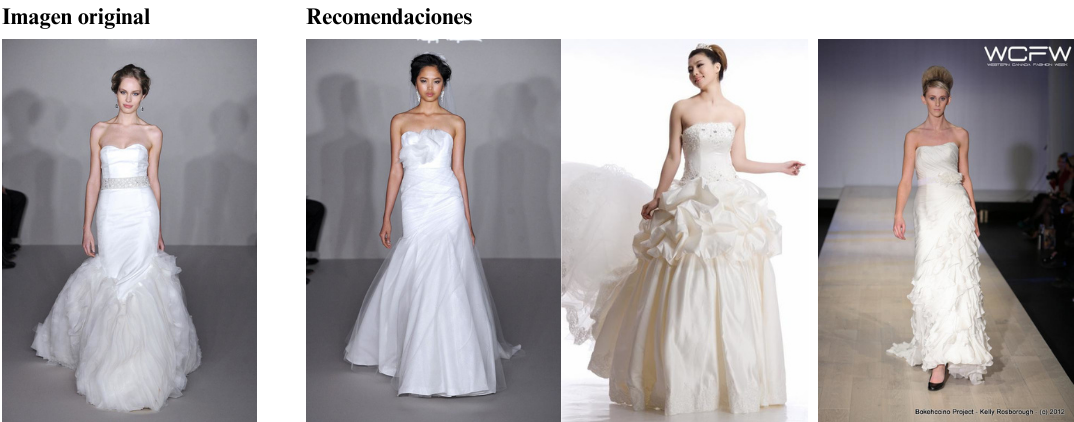
\includegraphics[scale=0.6]{recomendacion1.png}}
	\end{figure}
	\begin{table}[H]
		\centering
		\caption{Tabla de similitud de recomendaciones}
		\begin{tabular}{ll}
				\textbf{Recomendación} & \textbf{Similitud Coseno} \\
				\midrule
				Primera recomendación & 0,7575 \\
				Segunda recomendación & 0,7542 \\
				Tercera recomendación & 0,7465 \\
				\bottomrule
		\end{tabular}
	\end{table}
	\begin{figure}[H]
		\ffigbox[\FBwidth]
		{\caption{Recomendaciones sin uso de máscaras}}
		{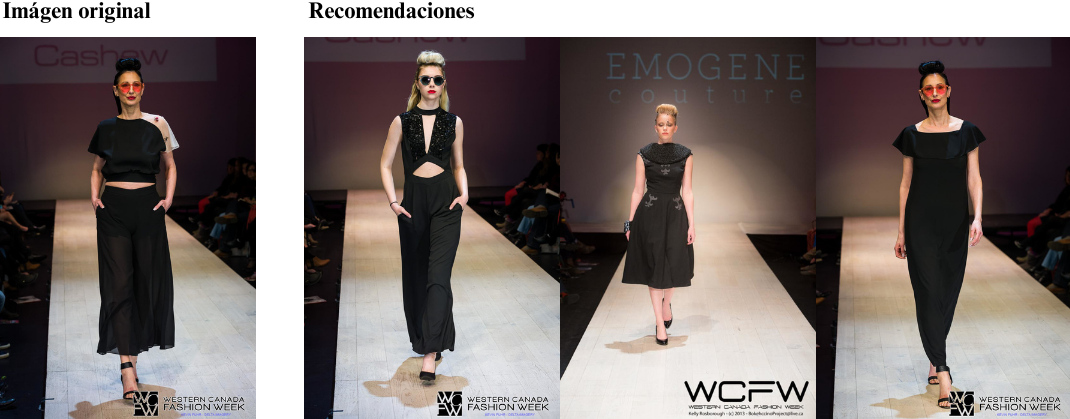
\includegraphics[scale=0.6]{recomendacion2.png}}
	\end{figure}
	\begin{table}[H]
		\centering
		\caption{Tabla de similitud de recomendaciones}
		\begin{tabular}{ll}
				\textbf{Recomendación} & \textbf{Similitud Coseno} \\
				\midrule
				Primera recomendación & 0,7951 \\
				Segunda recomendación & 0,7784 \\
				Tercera recomendación & 0,7723 \\
				\bottomrule
		\end{tabular}
	\end{table}
	Estas recomendaciones ejemplifican el problema presentado anteriormente. Todas ellas tienen una marca de agua en la
	esquina inferior derecha, todas ocurren en un desfile de moda, todas están vistiendo el color negro. Este hecho no impide
	que se obtengan porcentajes de similitud bastante altos, aun así el hecho de no hacer
	uso de las máscaras presenta los problemas descritos anteriormente.

	\section{Con máscaras}

	En este apartado se llevará a cabo un análisis similar al realizado en el anterior, pero esta vez haciendo uso de las máscaras.
	El hecho de utilizar máscaras reporta varios beneficios, entre ellos:
	\begin{itemize}
		\item Eliminar las recomendaciones basadas en el fondo de la imagen.
		\item Eliminar las recomendaciones basadas en el color de la prenda.
		\item Eliminar las recomendaciones basadas en el modelo que viste las prendas.
		\item Eliminar recomendaciones basadas en marcas de agua que pueda tener la imagen.
	\end{itemize}
	Es decir, las máscaras permiten al sistema recomendar únicamente en base a las prendas, sin tener en cuenta otros factores propios de las imágenes.
	A continuación, algunos ejemplos.

	\begin{figure}[H]
		\ffigbox[\FBwidth]
		{\caption{Recomendaciones con uso de máscaras}}
		{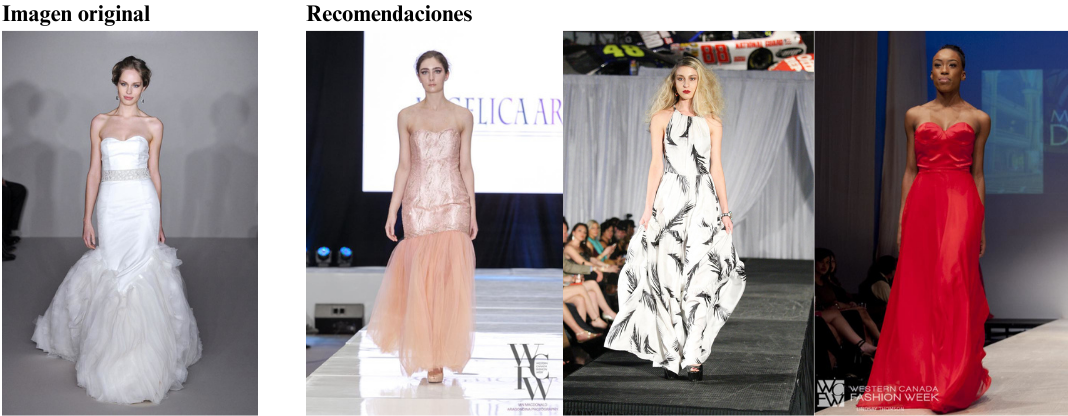
\includegraphics[scale=0.6]{recomendacion3.png}}
	\end{figure}
	\begin{table}[H]
		\centering
		\caption{Tabla de similitud de recomendaciones}
		\begin{tabular}{ll}
				\textbf{Recomendación} & \textbf{Similitud Coseno} \\
				\midrule
				Primera recomendación & 0,8856 \\
				Segunda recomendación & 0,8854 \\
				Tercera recomendación & 0,8657 \\
				\bottomrule
		\end{tabular}
	\end{table}

	\begin{figure}[H]
		\ffigbox[\FBwidth]
		{\caption{Recomendaciones con uso de máscaras}}
		{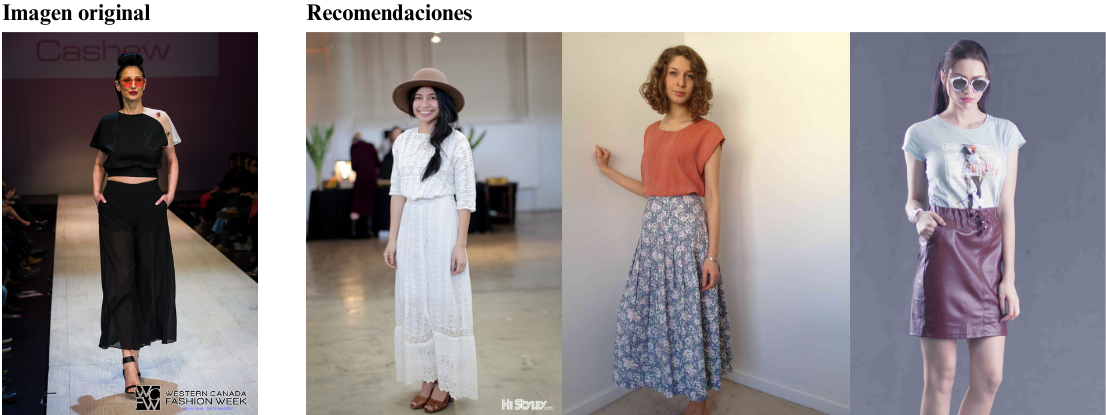
\includegraphics[scale=0.6]{recomendacion4.png}}
	\end{figure}
	\begin{table}[H]
		\centering
		\caption{Tabla de similitud de recomendaciones}
		\begin{tabular}{ll}
				\textbf{Recomendación} & \textbf{Similitud Coseno} \\
				\midrule
				Primera recomendación & 0,8899 \\
				Segunda recomendación & 0,8803 \\
				Tercera recomendación & 0,8766 \\
				\bottomrule
		\end{tabular}
	\end{table}

	Es fácil observar que los resultados de hacer uso de la máscara son claramente beneficiosos para el modelo de recomendación de imágenes.
	En primer lugar, las prendas recomendadas no tienen el mismo color que la original, tampoco la misma marca de agua o fondo. Además, los modelos
	no tienen ningún parecido entre sí. Otro indicador de la mejora de la recomendación es el porcentaje de similitud, que sube en torno al 10\%.
	Y, aunque puede tratarse de un aspecto subjetivo, las prendas son más parecidas entre sí, aunque no tengan el mismo color.

	\begin{figure}[H]
		\ffigbox[\FBwidth]
		{\caption{Gráfica de Similitud Coseno}}
		{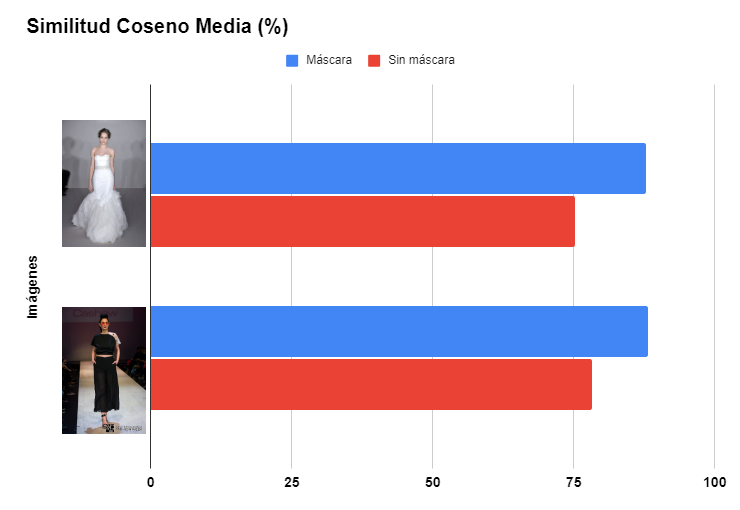
\includegraphics[scale=0.9]{grafica-similitud.png}}
	\end{figure}

	\begin{table}[H]
    \centering
    \caption{Medias de similitud coseno de imágenes}
    \begin{tabular}{lcc}
        & \multicolumn{2}{c}{Similitud Coseno Media} \\
        \cmidrule{2-3}
        & Con Máscara & Sin Máscara \\
        \midrule
        \multirow{2}{*}{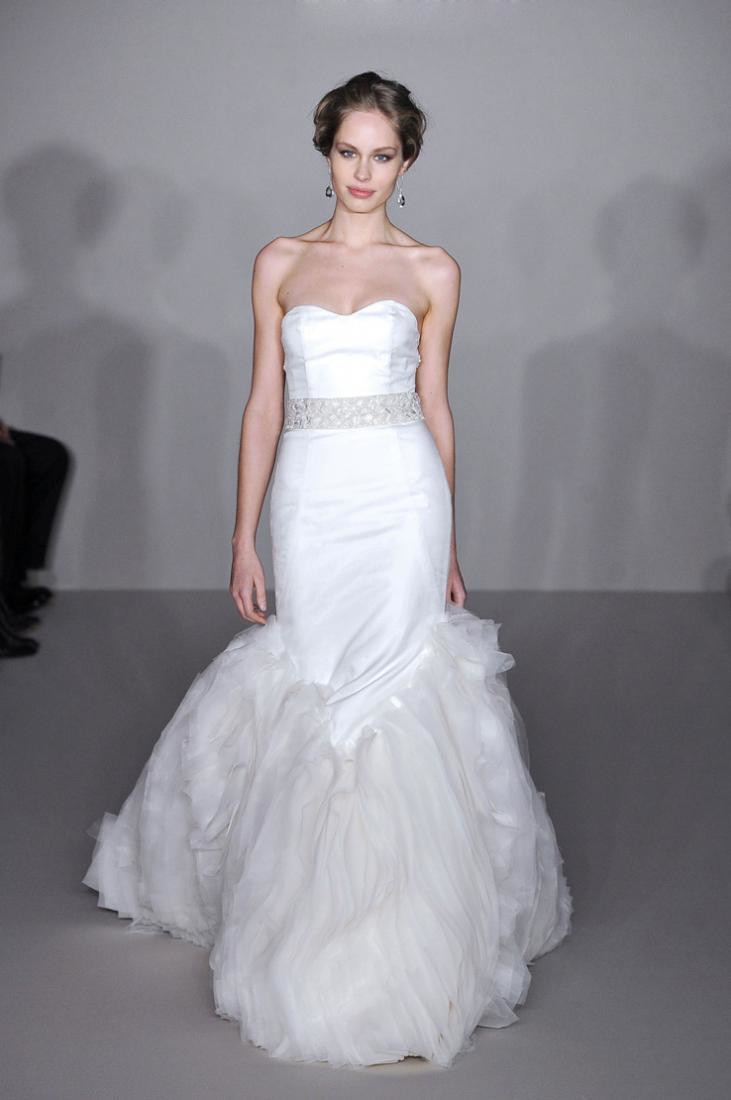
\includegraphics[width=0.8cm]{miniatura2.jpg}} & 0,8789 & 0,7527 \\
        &  &  \\
        \midrule
        \multirow{2}{*}{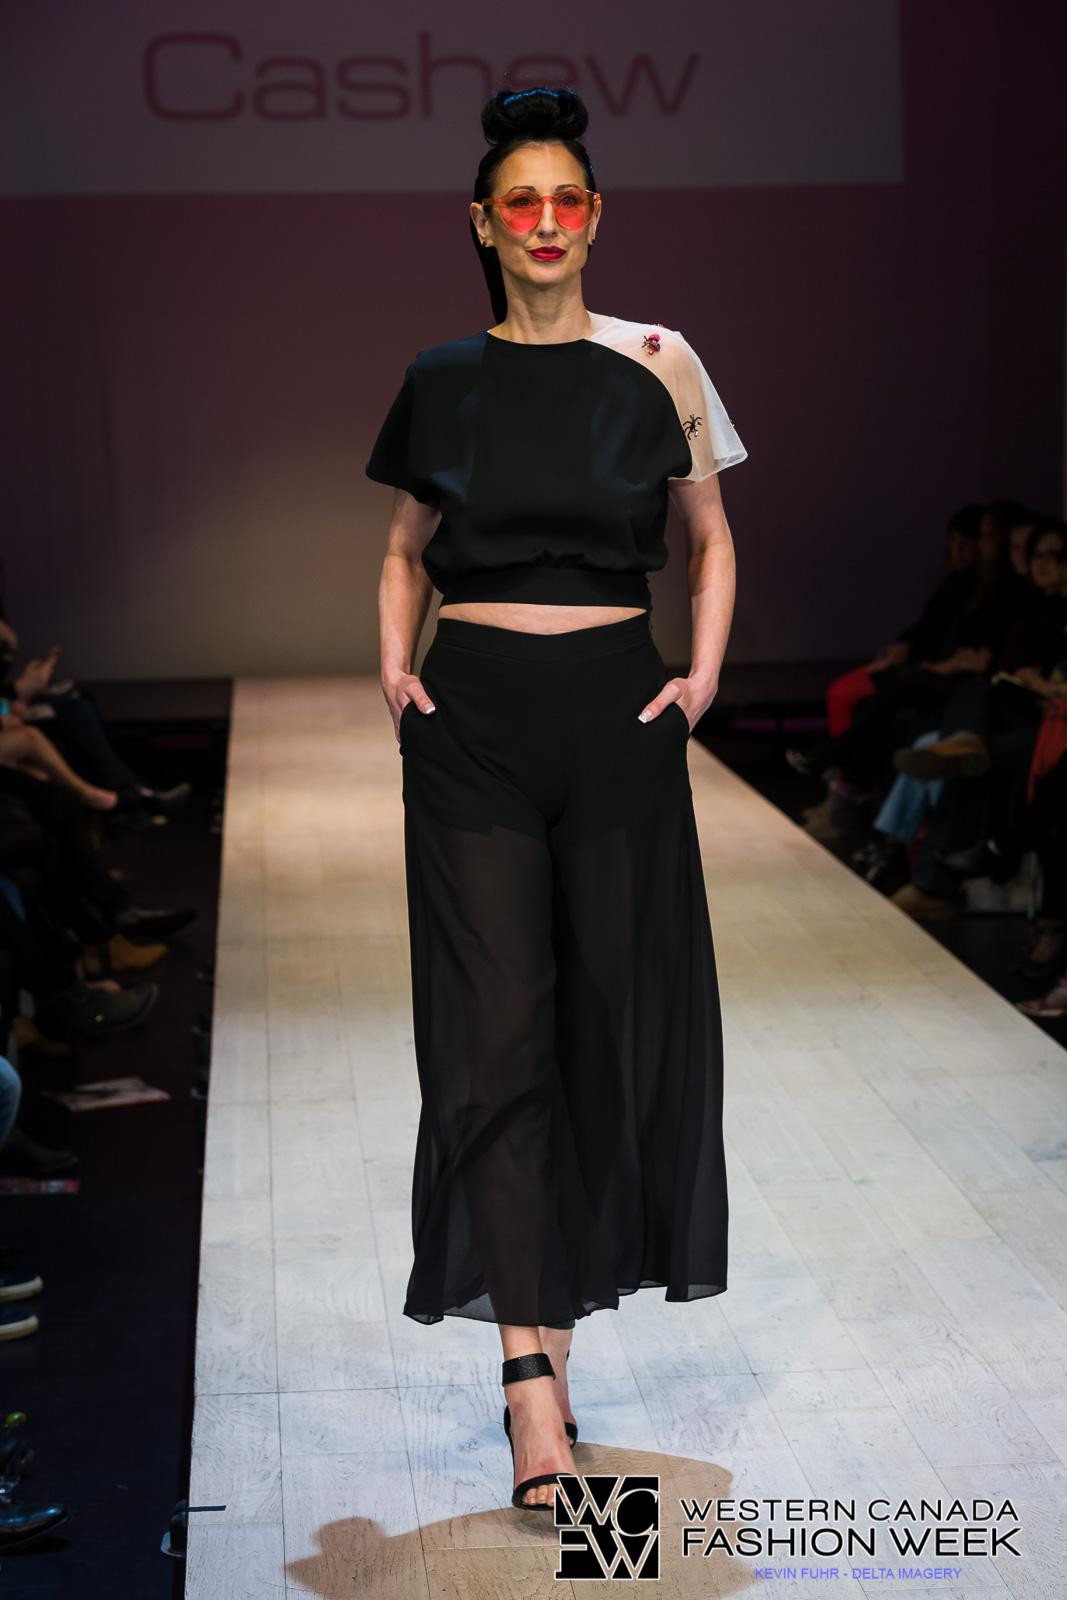
\includegraphics[width=0.8cm]{miniatura1.jpg}} & 0,8823 & 0,7819 \\
        &  &  \\
        \bottomrule
    \end{tabular}
	\end{table}

	\section{Uso de atributos}

	En este apartado se analiza el uso de los atributos en las recomendaciones y como estos afectan a la calidad
	de estas. En el siguiente ejemplo se selecciona el atributo ``blazer'' (chaqueta) para ejemplificar le uso de estos.
	\begin{figure}[H]
		\ffigbox[\FBwidth]
		{\caption{Recomendaciones con selección del atributo ``blazer''}}
		{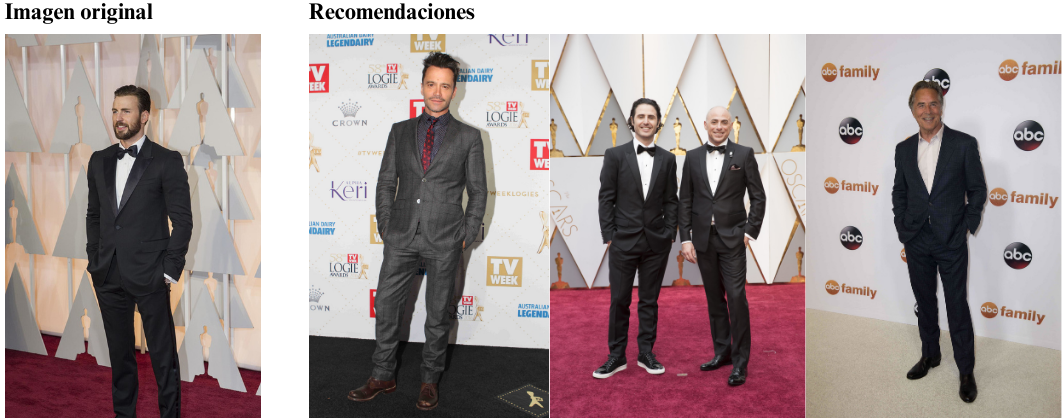
\includegraphics[scale=0.6]{atributos1.png}}
	\end{figure}
	\begin{table}[H]
		\centering
		\caption{Tabla de similitud de recomendaciones}
		\begin{tabular}{ll}
				\textbf{Recomendación} & \textbf{Similitud Coseno} \\
				\midrule
				Primera recomendación & 0,8779 \\
				Segunda recomendación & 0,8723 \\
				Tercera recomendación & 0,8679 \\
				\bottomrule
		\end{tabular}
	\end{table}
	
	Se puede observar que los porcentajes de similitud coseno siguen siendo buenos, a la altura de los anteriores. Además 
	podemos comprobar que todas las recomendaciones tienen el atributo ``blazer'' solicitado. 
	
	Ahora vamos a probar a añadir otro atributo a la consulta. Este atributo será ``loose (fit)''.
	\begin{figure}[H]
		\ffigbox[\FBwidth]
		{\caption{Recomendaciones con selección de los atributos ``blazer'' y ``loose (fit)''}}
		{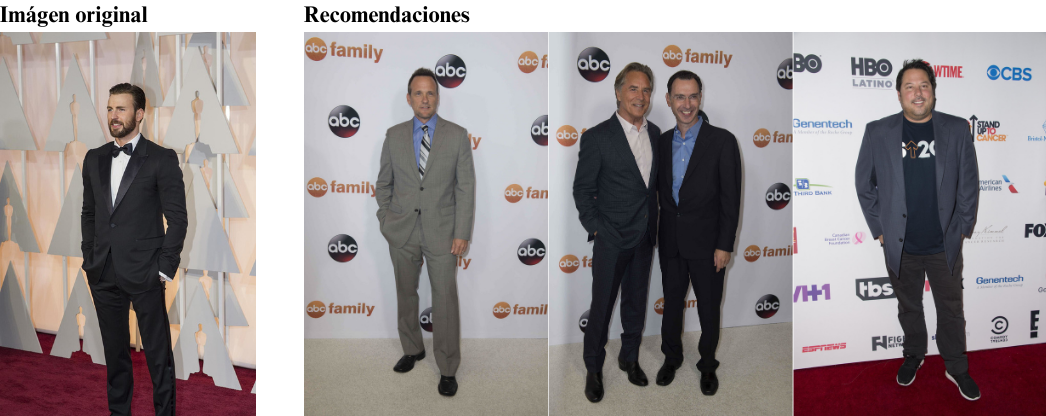
\includegraphics[scale=0.6]{atributos2.png}}
	\end{figure}
	\begin{table}[H]
		\centering
		\caption{Tabla de similitud de recomendaciones}
		\begin{tabular}{ll}
				\textbf{Recomendación} & \textbf{Similitud Coseno} \\
				\midrule
				Primera recomendación & 0,8406 \\
				Segunda recomendación & 0,8405 \\
				Tercera recomendación & 0,8357 \\
				\bottomrule
		\end{tabular}
	\end{table}

	Por último vamos a añadir el atributo ``geometric textile pattern''.

		\begin{figure}[H]
		\ffigbox[\FBwidth]
		{\caption{Recomendaciones con selección de los atributos ``blazer'' , ``loose (fit)'' y ``geometric textile pattern''}}
		{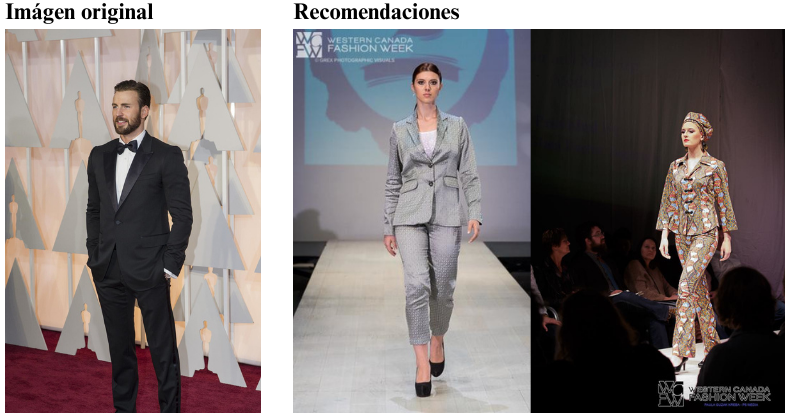
\includegraphics[scale=0.8]{atributos3.png}}
	\end{figure}
	\begin{table}[H]
		\centering
		\caption{Tabla de similitud de recomendaciones}
		\begin{tabular}{ll}
				\textbf{Recomendación} & \textbf{Similitud Coseno} \\
				\midrule
				Primera recomendación & 0,6712 \\
				Segunda recomendación & 0,5589 \\
				\bottomrule
		\end{tabular}
	\end{table}

	Como podemos comprobar a través de estos resultados, el uso de los atributos es un arma de doble filo. Resulta muy útil, pero se sacrifica porcentaje de similitud.
	Esto se debe a que cuantos más atributos queramos menos imágenes hay en el \textit{dataset} que contengan estos atributos, de hecho en el último ejemplo
	solo hay dos de ellas. Si tuvieramos un \textit{dataset} de un tamaño mucho mayor, como así sería en un ejemplo práctico en la vida real, este problema no se daría
	tan pronto. Aun así la selección de atributos resulta de gran utilidad.

	\chapter{Conclusiones}

	En este capítulo se llevarán a cabo las conclusiones generales del trabajo.
	Se hará un análisis que consistirá en comprobar si los objetivos iniciales han sido cumplidos.

	El objetivo principal de este trabajo era crear una interfaz gráfica que fuera capaz de recomendar imágenes de ropa
	a partir de, no solo una imagen dada por el usuario, sino también una serie de atributos deseados en esta recomendación.
	Este objetivo se ha podido cumplir por completo. Además se planteaban los siguientes sub-objetivos:
	\begin{itemize}
		\item Desarrollar un modelo de inteligencia artificial que sea capaz de recomendar imágenes en base a atributos multimodalaes y otra imagen.
		\item Crear una API que permita la comunicación entre el modelo previamente mencionado y una interfaz.
		\item Diseñar una interfaz intuitiva que permita a los usuarios cargar una imagen, seleccionar los atributos de interés y visualizar los resultados proporcionados por el modelo.
	\end{itemize}
	Se ha conseguido construir una aplicación web que lleva a cabo todas las tareas descritas anteriormente.

	La arquitectura VGG16 ha resultado ser útil para extraer las características de las imágenes. Esta ha sido efectiva y eficaz.
	El uso de máscaras, aunque haya ocasionado una solución más compleja debido a la tarea de segmentación, ha resultado aportar
	claras mejoras al modelo de recomendación. Las imágenes recomendadas dejan de estar influidas por aspectos ajenos a las prendas,
	como pueden ser el fondo de la imagen, marcas de agua o el aspecto físico de los modelos. Gracias a la combinación de la segmentación
	de las imágenes para la realización de las máscaras y la extracción de características de las imágenes, para el posterior cálculo de
	su similitud coseno, se ha podido llegar a obtener unos valores de similitud altos para las recomendaciones.

	El uso de los atributos también ha permitido al modelo filtrar el conjunto de datos y recomendar únicamente las prendas
	que contienen estos. Aun así, cuando se usan excesivos atributos juntos o se seleccionan algunos poco comunes, el modelo puede tener problemas
	recomendando debido al tamaño, no demasiado grande, del conjunto de datos.

	La principal limitación de este sistema de recomendación es el número de imágenes en el conjunto de datos. Añadir imágenes a este conjunto es costoso
	ya que se necesita ayuda de profesionales de la moda que clasifiquen correctamente los atributos de estas antes de añadirlas al conjunto. Además, cada vez
	que se añadan imágenes al conjunto de datos sería necesario volver a computar los vectores característicos, lo que puede hacer el proceso lento.
	Otra limitación de este trabajo es la posible falta de comprensión semántica de las imágenes por parte de la red neuronal. Esto puede provocar que en
	agunos casos las recomendaciones no sean las óptimas. Por último, este sistema cuenta con las limitaciones de no poder usar más de una única imagen como
	entrada para la recomendación ni permitir hacer una selección de colores deseados en esta.

	En conclusión, este trabajo cumple con los objetivos propuestos, brindando una interfaz que es capaz
	de servir un sistema de recomendación de imágenes con un alto porcentaje de similitud en las recomendaciones que aporta. Además, se ha podido introducir el uso de
	atributos, lo cual permite a los usuarios obtener recomendaciones más precisas y ajustadas a sus deseos. Si se contara con un conjunto de
	datos más grande esta última funcionalidad sería aún más precisa.

	\chapter{Trabajos futuros}
	
	Este trabajo tiene mucho margen de mejora y se pueden plantear
	una variedad de futuros trabajos a partir de este.

	En primer lugar, se puede Ampliar la base de datos sobre la que se trabaja, ya que a mayor cantidad de datos disponibles mayor será la calidad de 
	las recomendaciones. Esto ayudaría a corregir la limitación que se comentó en las conclusiones. Además, se podría llevar a cabo la
	implementación de una red neuronal más enfocada en la ropa y no tan generalista como la arquitectura VGG16. Entrenar una red que se centre en
	prendas en específico podrá ayudar a obtener mejores recomendaciones. 

	Con el fin de resolver la limitación de la falta de comprensión semántica de la red neuronal al extraer las carcterísticas de la imagen se podría añadir
	\textit{feedback} de usuarios reales durante el entrenamiento de la red. Esto podría ser de gran utilidad, ya que la calidad de las recomendaciones es muchas veces
	es subjetiva al gusto del usuario. 
	
	Otro posible trabajo futuro es permitir la posibilidad al usuario de utilizar la cámara del dispositivo desde el que se acceda a la aplicación web, 
	en lugar de tener que subir una foto ya hecha, para así hacer más fácil el uso de la interfaz. Además, se podría permitir subir varias imagenes,
	en lugar de solo una, para obtener resultados conjuntos. Por último, sería de gran utilidad permitir a los usuarios seleccionar los colores que desean
	obtener en sus recomendaciones.


	\chapter{Planificación y presupuestos}

	\section{Planificación}


	En este apartado se presenta la planificación que se ha llevado a cabo para la realización de este proyecto.
	La planificación ha consistido en las siguientes etapas:
	\begin{itemize}
		\item \textbf{Análisis del conjunto de datos.} 
		
		Esta etapa consistió en analizar el conjunto de datos, prepararlo para su uso y ver como se podía hacer uso de este. Se
		llevaron a cabo estadísticas que ayudaron al posterior diseño de la solución. Esta fase duró siete días.
		\item \textbf{Análisis de las técnicas posibles para la implementación del modelo y de la aplicación web.} 
		
		En esta etapa se analizan las diferentes tecnologías posibles para la resolución del problema. Se investiga
		cuales son las mejores técnicas para el modelo de segmentación, de extracción de características y se exploran las diferentes tecnologías web.
		Esta fase duró siete días.
		\item \textbf{Diseño de la solución.} 
		
		Se diseña la mejor solución a partir del análisis de tecnologías previamente hecho. Esta fase duró once días
		\item \textbf{Desarrollo, pruebas y mejoras.}
		
		Esta es la etapa más larga del proyecto, que consiste en el desarrollo. Una vez se finaliza el desarrollo
		del proyecto se itera a través de pruebas y se mejora la solución. 
		Esta fase duró cincuenta días.
		\item \textbf{Elaboración de la memoria.}
		
		Esta etapa consiste en documentar el trabajo realizado y duró treinta días.
	\end{itemize}

	Dadas estas etapas se puede estimar que el proyecto se ha elaborado en un total de 105 días. Cada uno de estos días se ha trabajado un total de
	ocho horas, lo que supone que el proyecto ha requerido 840 horas de trabajo. En la siguiente tabla se muestran las fechas detalladas
	de la planificación del proyecto.

	\begin{table}[H]
		\centering
		\caption{Planificación del proyecto}
		\begin{tabular}{llll}
				\toprule
				\textbf{Fase} & \textbf{Duración (días)} & \textbf{Inicio} & \textbf{Fin}\\
				\midrule
				\textbf{Análisis del conjunto de datos} & 7 & 15/05/2023 & 22/05/2023  \\
				\textbf{Análisis de técnicas y algoritmos} & 7 & 23/05/2023 & 30/05/2023 \\
				\textbf{Diseño de la solución} & 11 & 31/05/2023 & 11/06/2023 \\
				\textbf{Desarrollo, pruebas y mejoras} & 50 & 12/06/2023 & 31/07/2023 \\
				\textbf{Elaboración de la memoria} & 30 & 01/08/2023 & 31/08/2023 \\
				\bottomrule
		\end{tabular}
	\end{table}

	\section{Presupuestos}
	
	\subsection{Coste del personal}
	Este trabajo ha sido realizado por un solo ingeniero. Un ingeniero informático junior tiene un sueldo promedio en España
	de 2.208 €/mes \cite{sueldo}, lo que supone un sueldo de 13,8 €/hora. Se han trabajado ocho horas diarias por lo que el sueldo
	diario sería de 110,4 €.

	\begin{table}[H]
		\centering
		\caption{Planificación del proyecto}
		\begin{tabular}{llll}
				\toprule
				\textbf{Empleado} & \textbf{Días de trabajo} & \textbf{Sueldo diario} & \textbf{Coste total}\\
				\midrule
				Ingeniero junior & 105 & 110,4 € & 11.592 €  \\
				\bottomrule
		\end{tabular}
	\end{table}

	\subsection{Coste del equipo}
	El coste del equipo consiste en un ordenador de sobremesa y un portátil, teniendo en cuenta su uso.
	Para el cálculo del coste estimado teniendo en cuenta su uso se aplica la siguiente fórmula:

	\begin{equation}
		\text{Coste imputable} = \frac{\text{Tiempo de uso}}{\text{Tiempo de vida}} * \text{Coste total}
	\end{equation}

	\begin{itemize}
		\item \textbf{Ordenador de sobremesa}. Uso de ochenta horas con un coste total de 450 €
		\item \textbf{Portátil}. Uso de veinticinco horas con un coste total de 849,25 €
		\item \textbf{Teclado}. Uso de ochenta horas con un coste de 95 €
		\item \textbf{Monitor}. Uso de ochenta horas con un coste 240 €
	\end{itemize}

	\begin{table}[H]
		\centering
		\caption{Costes materiales}
		\begin{tabular}{lllll}
				\toprule
				\textbf{Concepto} & \textbf{Coste total (€)} & \textbf{Horas de uso} & \textbf{Tiempo de vida} & \textbf{Coste imputable (€)}\\
				\midrule
				Sobremesa & 450 & 80 & 1.200  & 30 \\
				Portátil & 849,25 & 25 & 800  & 26,54 \\
				Teclado & 95 & No aplica & No aplica  & 95 \\
				Monitor & 240 & No aplica & No aplica  & 240 \\
				\bottomrule
				\textbf{Total} & 1634,25 & & & 390,54
		\end{tabular}
	\end{table}

	\subsection{Costes directos}
	Los costes directos incluyen los costes del personal y los costes del equipo.
	\begin{table}[H]
		\centering
		\caption{Costes directos}
		\begin{tabular}{ll}
				\toprule
				\textbf{Descripción} & \textbf{Coste (€)}\\
				\midrule
				Costes de personal & 11.592  \\
				Costes de equipo & 390,54  \\
				\bottomrule
				\textbf{Total} & 11.982,54
		\end{tabular}
	\end{table}
	\subsection{Costes indirectos}
	Los costes indirectos incluyen gastos como agua, luz, gas, alquiler. Se estima que los costes indirectos son un 15\% del total
	de los costes directos, lo que supone un total de 1797,38 €.
	\subsection{Costes totales}

	Los costes totales son la suma de todos los costes descritos anteriormente.
	\begin{table}[H]
		\centering
		\caption{Costes directos}
		\begin{tabular}{ll}
				\toprule
				\textbf{Descripción} & \textbf{Coste (€)}\\
				\midrule
				Costes directos & 11.982,54  \\
				Costes indirectos & 1.797,38  \\
				\bottomrule
				\textbf{Total} & 13.779,92
		\end{tabular}
	\end{table}
	Por lo tanto se concluye que el coste total del proyecto estimado es de 13.779,92 €.


%	BIBLIOGRAFÍA
%----------	

\nocite{*} % Si quieres que aparezcan en la bibliografía todos los documentos que la componen (también los que no estén citados en el texto) descomenta está lína

\clearpage
\addcontentsline{toc}{chapter}{Bibliografía}
\setquotestyle[english]{british} % Cambiamos el tipo de cita porque en el estilo IEEE se usan las comillas inglesas.
\printbibliography



%----------
%	ANEXOS
%----------	

% Si tu trabajo incluye anexos, puedes descomentar las siguientes líneas
\chapter* {Anexo A: English summary}
\pagenumbering{gobble} % Las páginas de los anexos no se numeran

\section*{Introduction}
\section*{Work motivation}
The fashion industry has always been one of the most powerful in our society. This industry has been adapting to the rise of information technologies, and in the year 2022, online clothing sales accounted for 21.1\% of total sales in our country.

This is where recommendation systems come into play. A fashion recommendation system helps people find garments that align with their preferences. Customers can enhance their shopping experience and be content with their choices by receiving personalized and accurate recommendations. As a result, there is an increase in sales for fashion-focused websites. While an image-based recommendation system is useful, incorporating the option to specify garment attributes further enhances it.

Enabling users to receive recommendations saves them a significant amount of time that would otherwise be spent on potentially tedious searches. In conclusion, the creation of a multimodal attribute-based fashion recommendation system proves highly beneficial for both online store owners, as it improves their sales, and for users, who find it easier to locate the garments they are seeking, thus saving a considerable amount of time.
\section*{Objectives}

The goal of this work is to create a web interface capable of recommending clothing images with a certain similarity based on another image provided by the user. Additionally, users will be able to specify the attributes they desire in the output images (for example: long sleeves, loose fit, etc.).

With this being the primary objective, we can distinguish the following sub-objectives:
\begin{itemize}
	\item Develop an artificial intelligence model capable of recommending images based on multimodal attributes and another image.
	\item Create an API that facilitates communication between the aforementioned model and an interface.
	\item Design an intuitive interface that allows users to upload an image, select desired attributes, and view the results provided by the model.
\end{itemize}

These objectives aim to address the presented problem, resulting in a graphical web interface that empowers users to obtain clothing recommendations based on garments they like and the attributes they consider.

\section*{ Legal framework}

For the execution of this project, a set of images from the competition "iMaterialist (Fashion) 2020 at FGVC7" \cite{imaterialist} is utilized. These images contain real people's faces, so it is necessary to consider the Organic Law 3/2018 of December 5, regarding the Protection of Personal Data and the guarantee of digital rights \cite{ley-proteccion-datos}. Nonetheless, the dataset has been appropriately cited. For the same reason, attention must be paid to the Intellectual Property Law \cite{ley-propiedad-intelectual}. Furthermore, if we regard this as a research work, it would be necessary to take into account the Law 14/2011 of June 1, regarding Science, Technology, and Innovation \cite{ley-tecnologia}.

The tools used for the development of this project are open-source and freely available, such as Python, Visual Studio Code, Tensorflow, Keras, and React.

\section*{Socio-economic framework}

As mentioned previously in the motivation section, the fashion industry is one of the largest on a global scale. It generates significant interest and constitutes 2.8\% of the Spanish GDP and 4\% of the labor market \cite{estadisticas-moda}. This is why a fashion recommendation system holds great interest and social impact. Some of the benefits are as follows, according to Alma Muñoz's article ``How recommendation systems can help you achieve more sales'' \cite{alma}:
\begin{itemize}
	\item ``Between 15\% and 45\% increase in conversions.''
	\item ``25\% average increase in the average purchase value.''
	\item ``Extension of the customer's lifecycle.''
	\item ``Generation of buyer loyalty.''
\end{itemize}

Furthermore, Alma mentions that ``Amazon states that around 35\% of its revenue is attributed to product recommendations.''

Specifically, this product aims to be a fashion recommendation system. Therefore, it could be beneficial for any company engaged in online clothing sales due to the aforementioned benefits. Moreover, implementing this system on a clothing sales website provides a significant advantage over competitors.

A recommendation system also holds great societal relevance. Users of such systems can not only save substantial amounts of time but also discover garments more aligned with their taste and personality. This results in greater customer satisfaction, as they need to invest less time in finding better products.

In conclusion, this project offers numerous economic advantages for both sellers and buyers, saving time and achieving greater satisfaction with purchases. In the subsequent section, the planning and budget will be detailed.

\section*{Structure of the document}

The document is presented with a cover page, followed by an abstract along with keywords. Next, there is a general table of contents, a list of figures, and an acronym list. From here on, the document is divided into seven marked chapters:

\begin{itemize}
	\item \textbf{Introduction:} In this section, both the motivation for undertaking the work and the objectives it aims to achieve are presented. It also includes the regulatory framework and the socioeconomic context.
	\item \textbf{State of the Art:} An analysis of the current state related to the project's objective is elaborated upon. Similar works and the state of the employed technologies are examined. Additionally, the argument for how this project distinguishes itself from previously conducted works is provided.
	\item \textbf{System Design:} The solution to the proposed problem is explained, divided into its respective pre-established sub-objectives.
	\item \textbf{Results:} The obtained results are presented visually, with examples. Furthermore, their quality is analyzed using similarity percentages.
	\item \textbf{Conclusions:} A reflection that evaluates whether the proposed objectives have been met.
	\item \textbf{Future Work:} Possible continuations and improvements that can be undertaken based on this work are analyzed.
	\item \textbf{Planning and Budgets:} A summary of how the project has been planned and an explanation of the budget calculations are provided.
\end{itemize}

\section*{State of the art}
In this chapter, the current state of the project will be analyzed, taking a journey through the necessary technologies for its realization. Furthermore, an analysis of similar projects will be conducted, along with an argument regarding how this one can distinguish itself from them.

\section*{Computer vision}

Computer vision is the discipline of machine learning that deals with images. Through it, an attempt is made to computationally understand images. Among other things, computer vision is used for object recognition, image restoration, facial recognition, and a myriad of other tasks. Given that this project involves working with images, the importance of this discipline is paramount.

Computer vision has made significant progress in recent years, primarily due to improvements in hardware. We are now capable of performing a greater number of calculations on a larger amount of data, thanks to a significant increase in computing power. These advancements enable deeper investigation and exploration in this field.

With the advent of neural networks, it has become possible to perform complex tasks such as image classification, object detection, and segmentation. Convolutional neural networks have become the standard in this scientific field. They are capable of recognizing visual patterns that would be challenging, if not impossible, for a human to perceive.
\section*{Convolutional networks}
Neural networks are composed of different layers, which in turn are made up of different neurons. All networks have an input layer, one or more intermediate layers, and an output layer. The nodes in the layers are interconnected, and they can activate or not, depending on the outcome of their associated function, for the node to which they are connected.

Convolutional neural networks are the ones used for computer vision tasks. These networks are much more efficient when dealing with images, which is why they are employed in this field of machine learning. In the initial layers, elements of the image are identified at a larger scale, such as edges or colors. As the network goes deeper, larger parts of the image are recognized. Upon reaching the end, the network can identify the type of image. Convolutional networks consist of three layers:

\begin{itemize}
	\item \textbf{Convolutional Layer:} In this layer, the process known as convolution is applied. A filter (kernel) is used to detect the desired features in the image.
	\item \textbf{Pooling Layer:} In this layer, dimensionality reduction is applied. This layer is crucial because, although information is lost, efficiency is gained.
	\item \textbf{Fully Connected Layer:} In this layer, unlike the others, all nodes are connected to nodes in the previous layer.
\end{itemize}

There are several types of convolutional neural networks, including AlexNet, GoogleNet, ResNet, ZFNet, and VGGNet. For the completion of this project, the latter has been chosen.

\section*{Characteristics extraction}
For feature extraction, the VGG16 architecture has been chosen. This architecture was proposed by Karen Simonyan and Andrew Zisserman in the article titled ``VERY DEEP CONVOLUTIONAL NETWORKS FOR LARGE-SCALE IMAGE RECOGNITION'' \cite{vgg16-paper}.

This model achieved a 92.7\% accuracy on the ``ImageNet'' dataset, which contains over fourteen million images. It is one of the most popular models for working with feature extraction in images. It is highly useful for classifying images or, in the case of this project, calculating similarity between them.

The VGG16 architecture has been selected for several reasons. Firstly, it is extensively documented and easily accessible through \textit{Python} libraries. Despite being a simpler architecture than other options, it has been proven to have excellent performance in tasks related to computer vision, making it a solid choice for an image recommendation system. Furthermore, this architecture demonstrated its effectiveness in the article titled ``Image-based Product Recommendation System with Convolutional Neural Networks'' \cite{image-based-paper}.
\section*{Images segmentation}
When it comes to image segmentation, U2-Net stands out as the chosen architecture. Presented by researchers from a Canadian university in the year 2020, this architecture has rapidly gained prominence in the field of computer vision due to its high effectiveness.

U2-Net achieves highly precise segmentation by utilizing convolutional and deconvolutional layers, enabling it to capture features at a deep level. It has a remarkable ability to preserve fine details, making it well-suited for fashion image segmentation.

U2-Net is a leading architecture in the realm of image segmentation. Furthermore, its usage is straightforward in Python, and for these reasons, the decision has been made to employ it.
\section*{Similar work}
There are many previous works similar to this one. Among them, the following stand out:

\begin{itemize}
	\item ``Image-based Product Recommendation System with Convolutional Neural Networks'' \cite{stanford-paper}. This article describes the techniques used to create a recommendation system for online stores based on image similarity. The SVG, AlexNet, and VGG algorithms are tested. After evaluating all three, the latter proves to be the most accurate. Once image vectors are obtained, cosine distance is calculated between them to measure similarity.
	\item ``Image-Based Service Recommendation System: A JPEG-Coefficient RFs Approach'' \cite{image-based-paper}. This article consists of two phases. In the first phase, they classify images according to the type of product, while in the second, a recommendation system is created to find products most similar to a given one. For the second phase, which applies in our case, JPEG coefficients are used to extract image features. Subsequently, Euclidean distance is calculated between these coefficients.
\end{itemize}
This work differs in several aspects from the aforementioned ones. Not only does it seek recommendations based on an initial image, but it also allows users to select attributes they want the recommended images to have. In addition to this primary difference, this project goes beyond a mere model; it also includes a graphical interface that enables users to utilize the model.

\section*{System's design}
\section*{Dataset}
As mentioned in the ``Regulatory Framework'' section, this work utilizes the dataset ``iMaterialist (Fashion) 2020 at FGVC7'' \cite{imaterialist}. This dataset consists of several files, which are explained below.

Firstly, there are two sets of images: ``train'' and ``test''. The ``train'' set comprises 43,793 images, while the ``test'' set contains 3,200 images. Both sets include these images labeled with an identifier.
Additionally, there is a file named ``train.csv'' that contains the following fields:

\begin{itemize}
	\item \textbf{imageId:} Unique identifier for the images. For each image, there are multiple entries in the file, corresponding to the number of segmentations the image has.
	\item \textbf{encodedPixels:} These pixels represent the image segmentation.
	\item \textbf{height:} Height of the image.
	\item \textbf{width:} Width of the image.
	\item \textbf{classId:} Identifier of the class to which they belong.
	\item \textbf{attributesIds:} List of attribute identifiers contained in this image segment.
\end{itemize}

Segmentation is highly useful as it is used to create image masks. The ``attributesIds'' field is also noteworthy, as it allows us to filter images according to user preferences. These attributes are described in a file named ``label\textunderscore descriptions.json''. Each attribute has a description and a supercategory associated with its unique identifier.

\section*{Model}
\section*{Segmentation}
Firstly, the images need to be preprocessed. The objective of the task is to provide recommendations for similar clothing items, so anything other than clothing in the image can negatively impact the recommendation. For example, recommendations could include garments with a similar background in the image, images with the same watermark, or images where the models wearing them have physical similarities, among other things. These aspects should not influence the recommendation, which is why the first step is to create masks for the images. This is achieved using the ``encodedPixels'' attribute. These pixels, which represent the segmentation of the clothing, allow for the extraction of an image containing only the clothes.

However, this is not sufficient, as the user provides an image that is not in the database, meaning its segmentation is not available. Therefore, it is necessary to utilize a segmentation model to generate a mask for the user-provided image. There are numerous architectures that could address this issue. Some of them are described below:

\begin{itemize}
	\item \textbf{U-Net:} Named due to its U-shaped architecture, it combines convolutional and deconvolutional layers to achieve image segmentation.
	\item \textbf{SegNet:} Uses pooling layers to achieve image segmentation.
	\item \textbf{Mask R-CNN:} This architecture combines Faster R-CNN, used for object detection, with mask generation.
	\item \textbf{DeepLab:} Utilizes dilated convolution to achieve image segmentation.
	\item \textbf{U2-Net:} An extension of U-Net that includes mask generation.
\end{itemize}

Ultimately, the decision is made to use the U2-Net architecture, which encompasses all the advantages of U-Net and is additionally tailored for mask creation. This architecture demonstrates high accuracy even when dealing with high-resolution images, making it a strong candidate for fashion image segmentation.

U2-Net originated in 2020 at the University of Alberta, Canada, with the publication of the article ``U2-Net: Going Deeper with Nested U-Structure for Salient Object Detection'' \cite{u2net}. This article received recognition in 2020 as the best in pattern recognition.

\section*{Reccomendation algorithm}
The next step involves extracting features from all the images. To achieve this, a convolutional neural network is employed. As mentioned earlier, the decision has been made to use the VGG16 model. This model has an easily comprehensible structure and is deeper than its predecessors, such as AlexNet, enabling the extraction of more complex features.

The model utilizes the VGG16 architecture to extract the feature vector from all the masks. These vectors are stored in a matrix. When the user provides an image, its mask is generated using the previously mentioned procedure. Next, its feature vector is also obtained, and the cosine similarity is computed with the vectors from all other images. Finally, the dataset is filtered based on garments containing attributes selected by the user, and the top N images with the highest similarity are returned, where N is the desired number of images the user wants to obtain.

\section*{API}
In order to create a user-friendly graphical interface for the common user, it is necessary to have an API that serves the model. An API is a way to connect different applications to make them work together. The API enables the graphical interface to consume the previously described artificial intelligence model.

Python has been chosen for building this API, as it facilitates development since the model is also created using the same language. The chosen library for constructing this API is Flask, a framework designed for building CRUD applications (Create, Read, Update, Delete). A CRUD application can have multiple endpoints, which are routes to which a request can be sent. Each of these routes can perform actions like creating, reading, updating, or deleting information in the API.

For our API, only two endpoints have been necessary:

\begin{itemize}
	\item \textbf{``/recommendations'':}
	Uses the POST method. This endpoint expects to receive an image, a number of recommendations, and an optional list of attribute identifiers. Once it receives these arguments, the API utilizes the model and returns a list of image identifiers that, while having the required attributes, exhibit the highest similarity.
	\item \textbf{``/image/<id>'':}
	Through this endpoint, the API allows the retrieval of images based on their identifier, where ``id'' is the identifier of the desired image. It only requires a GET request with a valid identifier in the route.
\end{itemize}

\section*{Interface}
Several options were considered for the graphical interface. The first of these was StreamLit, a platform for developing interfaces for artificial intelligence projects written in Python. It enables the deployment of such applications in a very straightforward manner, requiring only a few lines of code. Additionally, Gradio was considered, which operates in a similar way to StreamLit. Both options are good, but in the end, the decision was made to use the React development framework, a JavaScript language. While the first two tools were interesting for achieving rapid development, they had limitations in terms of interface customization.

The inability to create the interface exactly as desired led me to choose React, which allows for building a complete web application from start to finish, including all its features. Furthermore, TypeScript is used instead of JavaScript for greater robustness due to its static typing. This helps prevent hard-to-debug errors during development, even though marking all the types may sometimes feel tedious. Using React proves highly advantageous as it allows for organizing code into reusable components where HTML and JavaScript come together.

The project has the following structure:

\begin{itemize}
	\item \textbf{``attributesSearch.tsx'':} This component is used to search for attributes that the user wants to select for their recommendations. It includes the complete list of attributes (selectable elements) and a search feature, given that there are 341 different attributes.
	\item \textbf{``attributesSelector.tsx'':} This component contains the attribute search. It also has a button that, if desired by the user, is used to obtain clothing recommendations with various attributes.
	\item \textbf{``header.tsx'':} This represents the page header.
	\item \textbf{``imageUploader'':} This component is a box that allows the user to upload the image they want to use for obtaining recommendations. It enables exploring local files and uploading an image file.
	\item \textbf{``stepper'':} This component is used to navigate through the screens of the information-giving process, as the application consists of a single page.
	\item \textbf{``services.ts'':} This file handles API requests.
	\item \textbf{``services.interfaces.ts'':} This file contains the necessary interfaces for the services.
	\item \textbf{``constants.js'':} In this file, variables that remain constant throughout the project are stored.
	\item \textbf{``globals.css'':} This file contains the CSS configuration that affects the entire project.
	\item \textbf{``label\textunderscore descriptions.json'':} This file is used to associate attribute identifiers with their descriptions.
	\item \textbf{``page.tsx'':} This is the main page where all the components come together to compose the application.
\end{itemize}

Upon loading the page, a window prompts us to upload an image. Once the image is uploaded, you can press the ``Next'' button, which takes you to selecting the number of recommendations through a number selection bar. Once again, you can press the ``Next'' button; this time, it leads you to the final window, the attribute selection. This window contains the complete list of selectable attributes. Selected attributes are marked at the top, where they can be deselected. Additionally, there is a search bar given the large number of attributes. Once everything is set, you can press the ``Process'' button. This button sends a request to the API which, utilizing the model, returns the identifiers of the most similar images. With these identifiers, a request is made for each of them to obtain their respective images. These images are displayed in a gallery that can be viewed in full size. If you wish to repeat the process, you can simply press the ``Reset'' button.

\section*{Conclusions}
In this chapter, we will present the overall conclusions of the work carried out. An analysis will be conducted to verify the fulfillment of the initial objectives. The main objective of this work was to create a graphical interface capable of recommending clothing images based not only on a user-provided image but also on a set of desired attributes for the recommendation. This objective has been fully achieved. Additionally, the following sub-objectives were outlined:

\begin{itemize}
	\item Develop an artificial intelligence model capable of recommending images based on multimodal attributes and another image.
	\item Label the images to be used with their respective attributes.
	\item Create an API that allows communication between the aforementioned model and an interface.
	\item Design an intuitive interface that enables users to upload an image, select attributes of interest, and visualize the results provided by the model.
\end{itemize}

A web application has been successfully built to perform the tasks described above, leading to the conclusion that the work has been successful.

The VGG16 architecture has proven to be useful for extracting image features. It has been effective and efficient. The use of masks, although leading to a more complex solution due to the segmentation task, has clearly improved the recommendation model. Recommended images are no longer influenced by elements unrelated to the garments, such as image backgrounds, watermarks, or the physical appearance of models. Through the combination of image segmentation for mask creation and feature extraction for subsequent cosine similarity calculation, very good similarity percentages have been achieved for recommendations.

The use of attributes has also been successful. The model is capable of filtering the dataset and recommending only garments that possess these attributes. However, when an excessive number of attributes are used together or some uncommon attributes are selected, the model may encounter recommendation challenges due to the not overly large size of the dataset.

In conclusion, this work has been successful, as it has perfectly fulfilled the proposed objectives, providing a clean interface capable of serving an image recommendation system with a high percentage of similarity in the provided recommendations. Furthermore, the use of attributes has been integrated, allowing users to obtain more precise and tailored recommendations. If a larger dataset were available, this latter functionality would be even more accurate.

\section*{Future work}
The field of computer vision could be considered relatively new. Therefore, there is significant room for improvement, and a variety of future work can be proposed from this point. Some of these possibilities include:
\begin{itemize}
	\item Expanding the working database, as having a greater quantity of available data will lead to higher-quality recommendations.
	\item Implementing a neural network more focused on clothing and less generalized than the VGG16 architecture. Training a network specifically tailored to clothing could enhance recommendation quality.
	\item Incorporating feedback from real users during network training could be highly beneficial, as recommendation quality is often subjective and depends on user preferences.
	\item Exploring the possibility of utilizing the device's camera when accessing the web application to facilitate the recommendation process.
	\item Allowing users to provide multiple images to obtain collective results.
	\item Enabling users to select colors for their recommendations.
\end{itemize}

These potential directions could contribute to advancing the field of computer vision for fashion and enhancing the capabilities of the recommendation system.
\end{document}